\documentclass[type=dr, dr=rernat, accentcolor=tud7b,colorbacktitle, bigchapter, openright, twoside, 12pt ]{tudthesis}
%\documentclass[11pt,twoside,a4paper]{article}
\usepackage[english]{babel} 
\usepackage[utf8]{inputenc}
\usepackage{graphicx}
\usepackage{pstricks}
\usepackage{psfrag}
\usepackage{enumerate}
\usepackage{float}
\usepackage{epsfig}
\usepackage{geometry}
\usepackage{subfigure}
\usepackage{rotating}
\usepackage{minitoc}
%\usepackage{appendix}

%%%% 1 1/2 facher Zeilenabstand:	
\usepackage{setspace}
\onehalfspacing




\begin{document}
\chapter{Introduction - research background and fundamentals}
\label{chapter:intro}
\minitoc

\section{Radiotherapy}

An ionizing radiation was used for treating tumors since the discovery of X-rays in 1895. In the beginning only superficial diseases would be treated, but as time and technology progressed X-ray tubes gained on voltage, allowing treatment of deeper seated tumors.

The radiation from linear accelerator was first used in medicine in 1953. Because the beam is more collimated and energies are
higher compared to X-ray tubes, the cure rates improved tremendously. The next big milestone was introduction of computers in the field
of radiotherapy. This led to better diagnostic tools, such as computed tomography scans (CT), magnetic resonance imaging (MRI) and
positron emission tomography (PET). With these tools the location of the tumor could be better estimated and hence the physicians
could prescribe better treatment. The potential of computers was afterwards exploited also in the treatment planning process, resulting in intensity modulated
radiation therapy (IMRT) which, together with diagnostic tools, provides an exact dose shaping in accordance to patient specific tumors.

In 1946, a paper from R. Wilson first described the application of protons for cancer treatment \cite{Wilson1946}. It was shown that protons have preferable depth dose profile compared to photons. First patient treatment soon followed in the early 1950's at Lawrence Berkeley Laboratory, USA. Heavier ions, such as 
$^{2}$He, $^{20}$Ne and $^6$C were later also used for treatment. In the beginning only passive beam delivery (see Section \ref{Sec::Passive}) was used for treatment and in the 1990's active beam solutions (see Section \ref{Sec::Active}) were developed at Paul Scherrer Institute (PSI), Villigen (Switzerland) for protons and at GSI, Darmstadt (Germany) for carbon ions.


\section{Physical and biological basics of radiotherapy}

The aim of radiotherapy is to kill tumor cells and prevent further growth, while sparing healthy tissue. Both radiotherapy modalities (photons and ions) use the same principle to eliminate cancer cells - 
they aim to damage the cell genetic material through ionization. The actual physical and biological mechanism behind both modalities will be explained in detail in the following section.

\subsection{Interaction of radiation with matter}

The interactions between photons with matter and ions with matter are quite different, as can be seen from depth dose distributions in Fig.~\ref{ddp}. Photons deposit the highest local dose shortly after entering the matter 
(at the energies used in radiotherapy). Ions, on the other hand, deposit most of their dose right before they stop in the so-called Bragg Peak region. The position of the Bragg Peak depends on the energy of the ions, which is exploited in the treatment
of deep suited tumors.

\subsubsection{Dose definition}

An important quantity in radiotherapy is dose, $D$, defined as the ratio of the absorbed energy $dE$ per mass element $dm$ \cite{ICRU1993}:

\begin{equation}
 D = \frac{dE}{dm} \quad \left[ Gy = \frac{J}{kg} \right]
\end{equation}

Usually we can describe energy loss of a beam in a thin layer of material, $dE/dx$. Dose can be then rewritten as:

\begin{equation}
 D = \frac{dE}{dx} \times \frac{1}{F} \times \frac{1}{\rho}
\end{equation}

where $F$ is the fluence and $\rho$ the material density.


\newpage

\begin{figure}[H]
\begin{center}
% 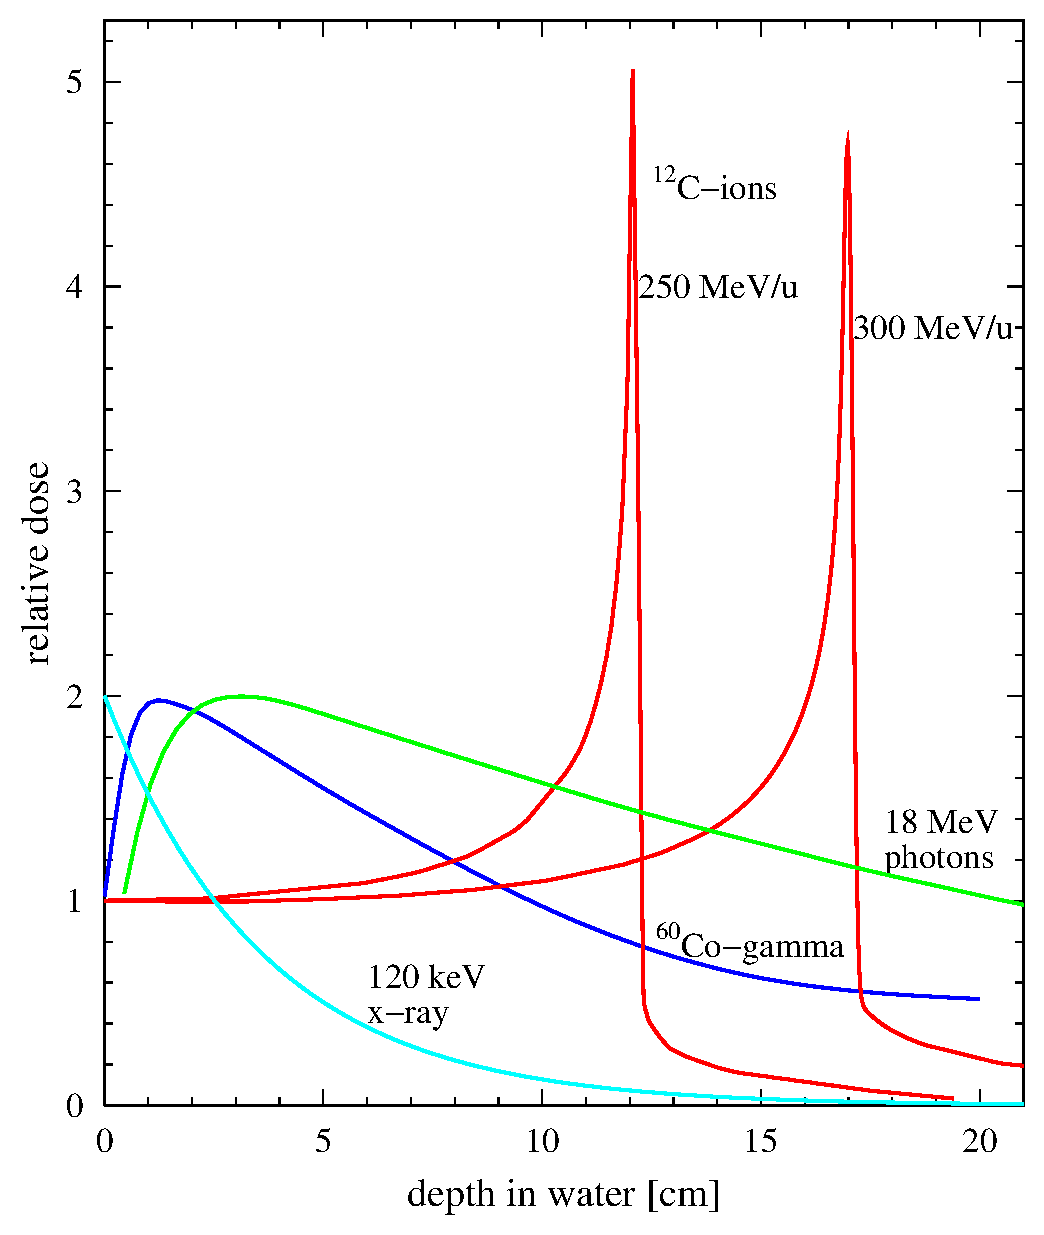
\includegraphics[scale=1]{depthdose.eps}
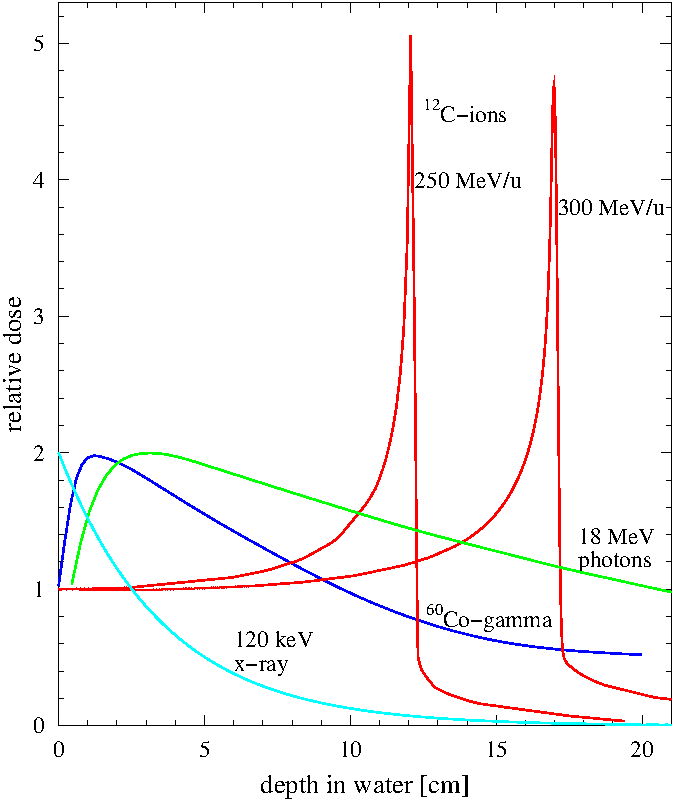
\includegraphics[width=0.9\textwidth]{./Images/depthdose.png}
\caption{Photon and carbon ions depth dose distributions at different energies. Photons start with a build up, which is then followed by an exponential decrease. Ions deposit most of the dose at the end of the particle track - the Bragg peak. Figure taken from \cite{Schardt2010} }
\label{ddp}
\end{center}
\end{figure}

\subsubsection{Interaction of photons with matter}

Photons mostly interact with matter in one of the following ways: coherent or Rayleigh scattering, photoelectric effect, Compton scattering and pair production. The cross section $\sigma$, for each of these processes depends as well on the energy of the incident photons as on the atomic number of the absorbing material \cite{Lilley2006}. The decreasing photon intensity in matter, $I$, can be described as:

\begin{equation}
 I = I_{0} \cdot e^{- N \sigma x} = I_{0} \cdot e^{-\mu x}
 \label{expdecrease}
\end{equation} 

where $I_{0}$ stands for the initial intensity of the photons, $x$ the depth of the material in units of length, $N$ the atomic density of the material and $\mu$ the attenuation coefficient. The cross section, $\sigma$ is the sum of all possible Interaction processes:

\begin{equation}
{\sigma} = \sigma_{rayleigh} + \sigma_{photoelectric} + Z\sigma_{compton} + \sigma_{pairproduction} 
\end{equation}
The energy range of photons used in radiotherapy is between 100 keV and 25 MeV. The dominating process in this energy range is Compton scattering \cite{Alpen1998}.
The electrons resulting from Compton interaction scatter mostly in a forward direction. Therefore a maximum of the depth-dose profile occurs when electrons stop at a certain depth, 
the mean electron range. After this build up the dose deposition decreases exponentially (see Fig.~\ref{ddp} and Equation \ref{expdecrease}).

\subsubsection{Interaction of ions with matter}
\label{iion}
Ions can interact with matter either with elastic Coloumb scattering from target nuclei (nuclear stopping) or with inelastic collision with target electrons (electronic stopping).
At the ion energies used in radiotherapy, which are less then 500$\mathrm{MeV}/\mathrm{u}$, the electronic stopping is the dominating interaction. The result is ionization and excitation of the target atoms.

The mean rate of the ions energy loss in matter is described by the Bethe-Bloch formula \cite{Bethe1930, Bloch1933}. Since we are interested in low ion energies, a non-relativistic approximation ca be made:

\begin{equation}
- \left \langle \frac{dE}{dx} \right \rangle = \frac{ 4 \pi N_{e} z_{eff}^{2} }{ m_{e} v^{2} } \left( \frac{e^{2}}{4\pi \epsilon_{0}} \right) ^{2} \left[ln \left( \frac{2m_{e}v^{2}}{I} \right)+correction \right]
 \label{bethe}
\end{equation}



here $N_{e}$ is the material's electron density, $e$ and $m_{e}$ are the charge and mass 
of an electron, $\epsilon_{0}$ the electrical field constant and $I$ the mean excitation energy of the absorber material. 
Barkas formula \cite{Barkas1963} can be used for the approximation of the effective projectile charge $z_{eff}$: 

% \vspace*{-0.8cm}
\begin{equation}
 z_{eff} = z \left( 1 - e^{-125 \beta z^{\frac{2}{3}}} \right)
\end{equation}

where $\beta$ is the projectile speed in units of $c$.

The energy loss of the ions is proportional to $z_{eff}$ and inversely proportional to $v^2$. The shape of the curve in Fig.~\ref{ddp} can be explained as following: Ions enter the matter with a high velocity, resulting in a small energy deposition. Their velocity gradually decreases, which in turn increases the energy deposition. The maximum of the energy loss occurs right when the ions stop and it is called Bragg peak.

\subsubsection{Lateral scattering and range straggling of ions}
\label{scat}
As mentioned ions interact with matter mostly via electronic stopping at energies used in radiotherapy. However, nuclear stopping still occurs and it is the main reason for lateral scattering.
The angular spread of ions is dependent on the mass of the target nuclei and on the momentum of the incident ions \cite{Moliere1948}. The lateral scattering is proportional to the mass of the target nuclei and inversely proportional
to the momentum of incident ions. Carbon ions have thus less lateral scattering then protons. Experiments have shown that carbon ions have three times smaller angular spread compared to protons at the same range in water 
(15.6 cm, 150 MeV/u protons and 285 MeV/u $^{12}$C ions) \cite{Schardt2010}.

Statistical fluctuations of specific electronic stopping events cause range straggling of ions. If the number of collisions is high or the material is thick enough these fluctuations can be approximated by
a Gaussian probability distribution \cite{Bohr1940, Ahlen1980}. The straggling width $\sigma_R$ is proportional to:

\begin{equation}
 \sigma_R \propto R/\sqrt{M}
\end{equation}

where $R$ is the mean range of ions and $M$ the ion mass. Thus, the heavier the ion is, the less range straggling it has. Carbon ions have 3.5 smaller range straggling when compared to protons \cite{Schardt2010}.

\subsubsection{Nuclear fragmentation}
\label{nuclfrag}

When transversing through matter ions (except protons) can be fragmented into ions with lower atomic number. The lower Z fragments travel in the same direction as projectile ions and 
have a significant contribution to the deposited dose (see Fig.~\ref{iondd}). It is thus essential that fragments are included in the treatment planning, so that an accurate dose can be calculated.

After colliding with the target projectile fragments enter excited state. A de-excitation occurs through
emission of nucleons, nucleon clusters and photons. Two of the possible fragments of projectile $^{12}$C ions are isotopes $^{11}C$ and $^{10}C$, which are both $\beta^+$ emitters \cite{Kraft2000}.
The resulting positron is annihilated with electrons in matter, creating two photons, which travel in opposite direction. PET (Positron Emission Tomography) can take advantage of the process without exposing patient to additional radiation.

\begin{figure}[H]
\begin{center}
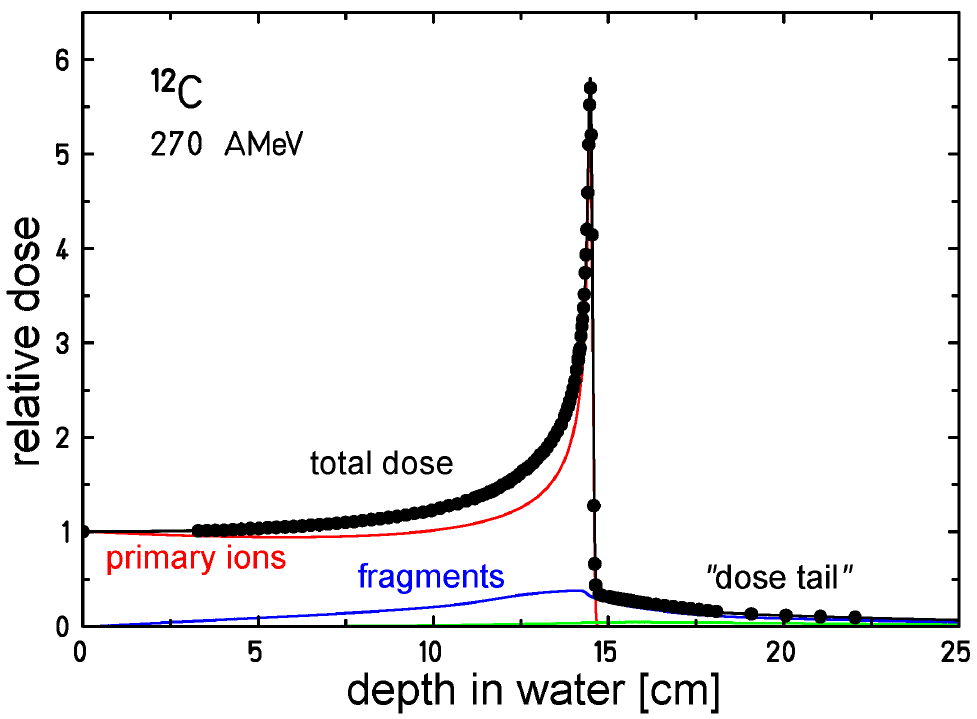
\includegraphics[width=0.7\textwidth]{./Images/iondepthdosesum.png}
\caption{Impact of fragmentation on a depth dose distribution of carbon ions. Main contribution to the overall deposited dose (black line) comes from the primary ions (red line). The produced fragments 
(blue line) have a smaller impact, but non-negligible. The most profound effect is seen in the dose tail behind the Bragg peak, where dose comes only from fragments. Figure taken from \cite{Groezinger2004}}
\label{iondd}
\end{center}
\end{figure}

\subsubsection{Secondary electrons and track structure}

Ions used in radiotherapy loose most of their energy via inelastic Coulomb scattering on target electrons. Electrons liberated from target by ions are called secondary electrons or $\delta$-electrons. 
$\delta$-electrons travel through matter, scatter further and may produce secondary ionization of the target atoms. When $\delta$-electrons energies are larger than $>$50 eV,
ionization becomes the dominant process, which produces a large number of additional electrons \cite{Kraft2000,Schardt2010}.

The radial dose profile and track diameter is defined by the energy spectrum of the $\delta$-electrons. Most of the $\delta$-electrons are concentrated around the projectile ions path, since they receive small energy transfers 
or are scattered in the direction of incident ions. Different models \cite{Chatterjee1976,Katz1999} and Monte Carlo simulations \cite{Paretzke1986,Kraemer1995} predict radial dose fall-off approximately with $1/r^2$ for radial distance $r$. Varma et. al. have confirmed 
this experimentally \cite{Varma1977}. The maximum radial distance $r_{max}$ is defined by the most energetic $\delta$-electrons, which are related to energy, $E$, of the projectile ions \cite{Kiefer1986}.

\begin{equation}
 r_{max} = E^{1.7}
\end{equation}

Following equation \ref{bethe}, $E$ is correlated to $Z^2$ and $1/\beta^2$, meaning that track structure is highly dependent on the projectile ion species and energy as demonstrated in Fig.~\ref{track}:
Carbon ions have much more dense ionization structure compared to protons \cite{Kraemer2010}. $\delta$-electrons have low energies, and thus the $r$ is on nanometer scale. As the energy of projectile ions decreases, their
stopping power increases and causes significantly larger number of $\delta$-electrons. The energy deposited by $\delta$-electrons in medium is described using the Linear Energy Transfer (LET), which is closely related to 
$dE/dx$. Fast ions, with little ionization, have thus small LET, while slow ions, with large ionization, have a high LET.


\subsection{Radiobiology}

Ionizing radiation (photons and ions) causes damage throughout the cell. However the most susceptible part to radiation is the
carrier of genetic information, the deoxyribonucleic acid (DNA), located in the cell nucleus \cite{Munro1970}. Radiation can damage DNA directly or indirectly.

Ionization and consequent destruction of DNA molecular bonds via radiation is a direct effect (see Fig.~\ref{ida}b) and is typical for high-LET radiation. On the other hand, an indirect effect is when radiation hydrolysis water around DNA and produce highly reactive hydroxyl-radicals, OH 
(see Fig.~\ref{ida}a). Even though OH radicals decay fast, they are still able to cause severe damage to DNA. The formation of OH is typical for low-LET radiation like photons. The two processes, direct and indirect, are not exclusive and can damage DNA in parallel.


\newpage

\begin{figure}[H]
\begin{center}
% 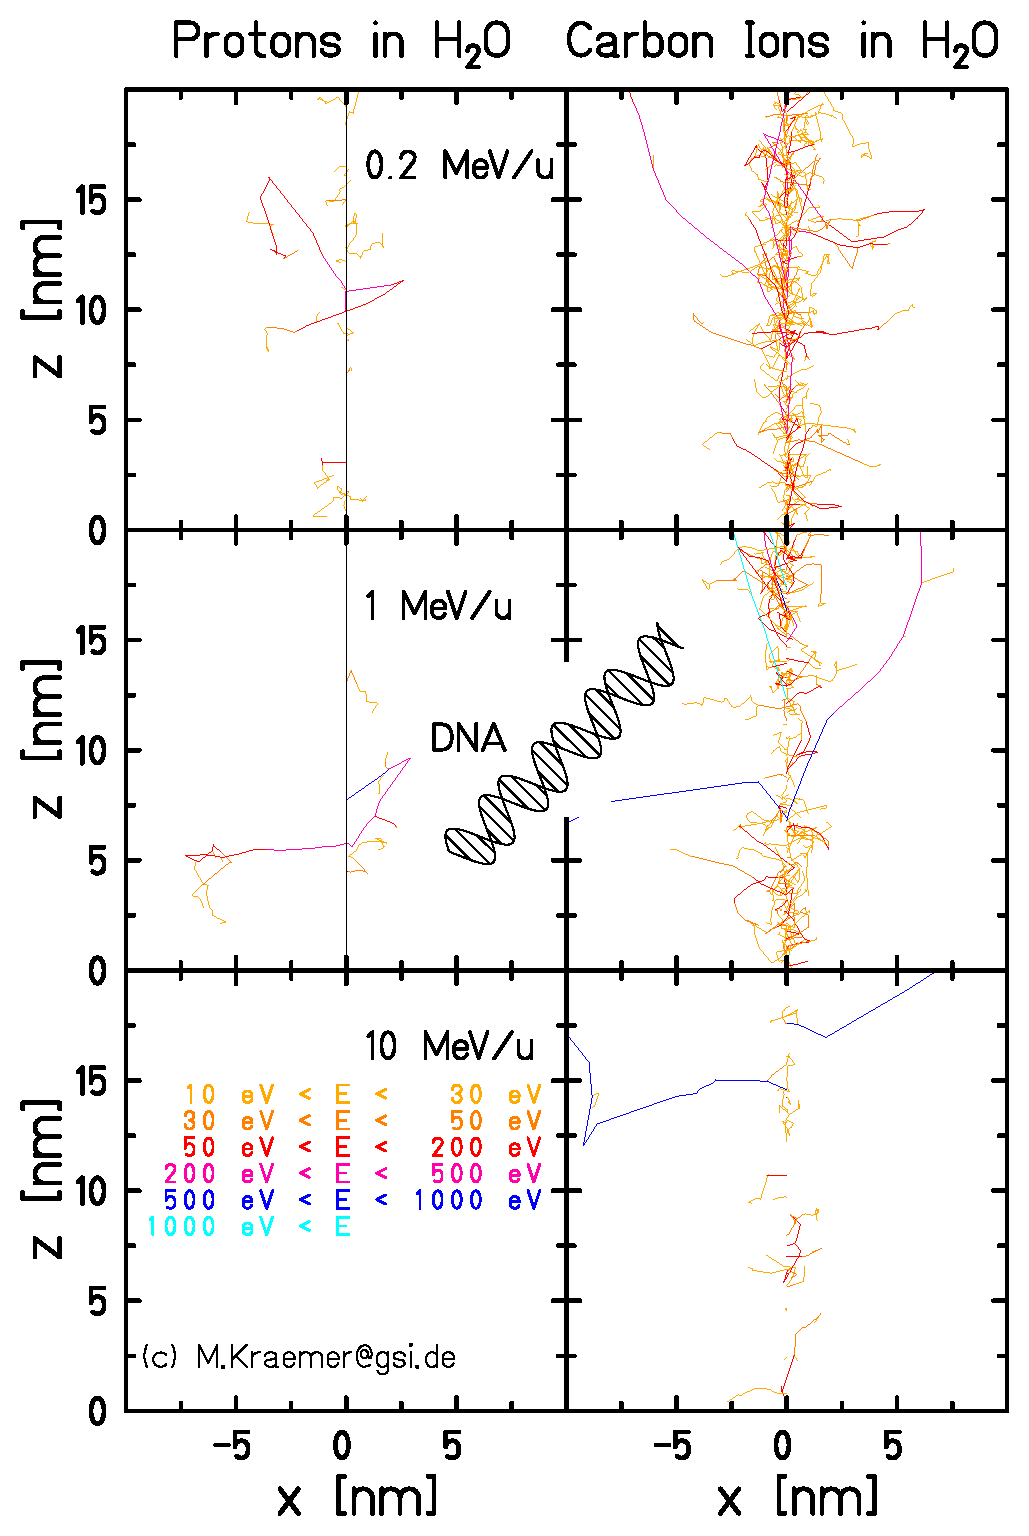
\includegraphics[scale=0.75]{trackstructure.eps}
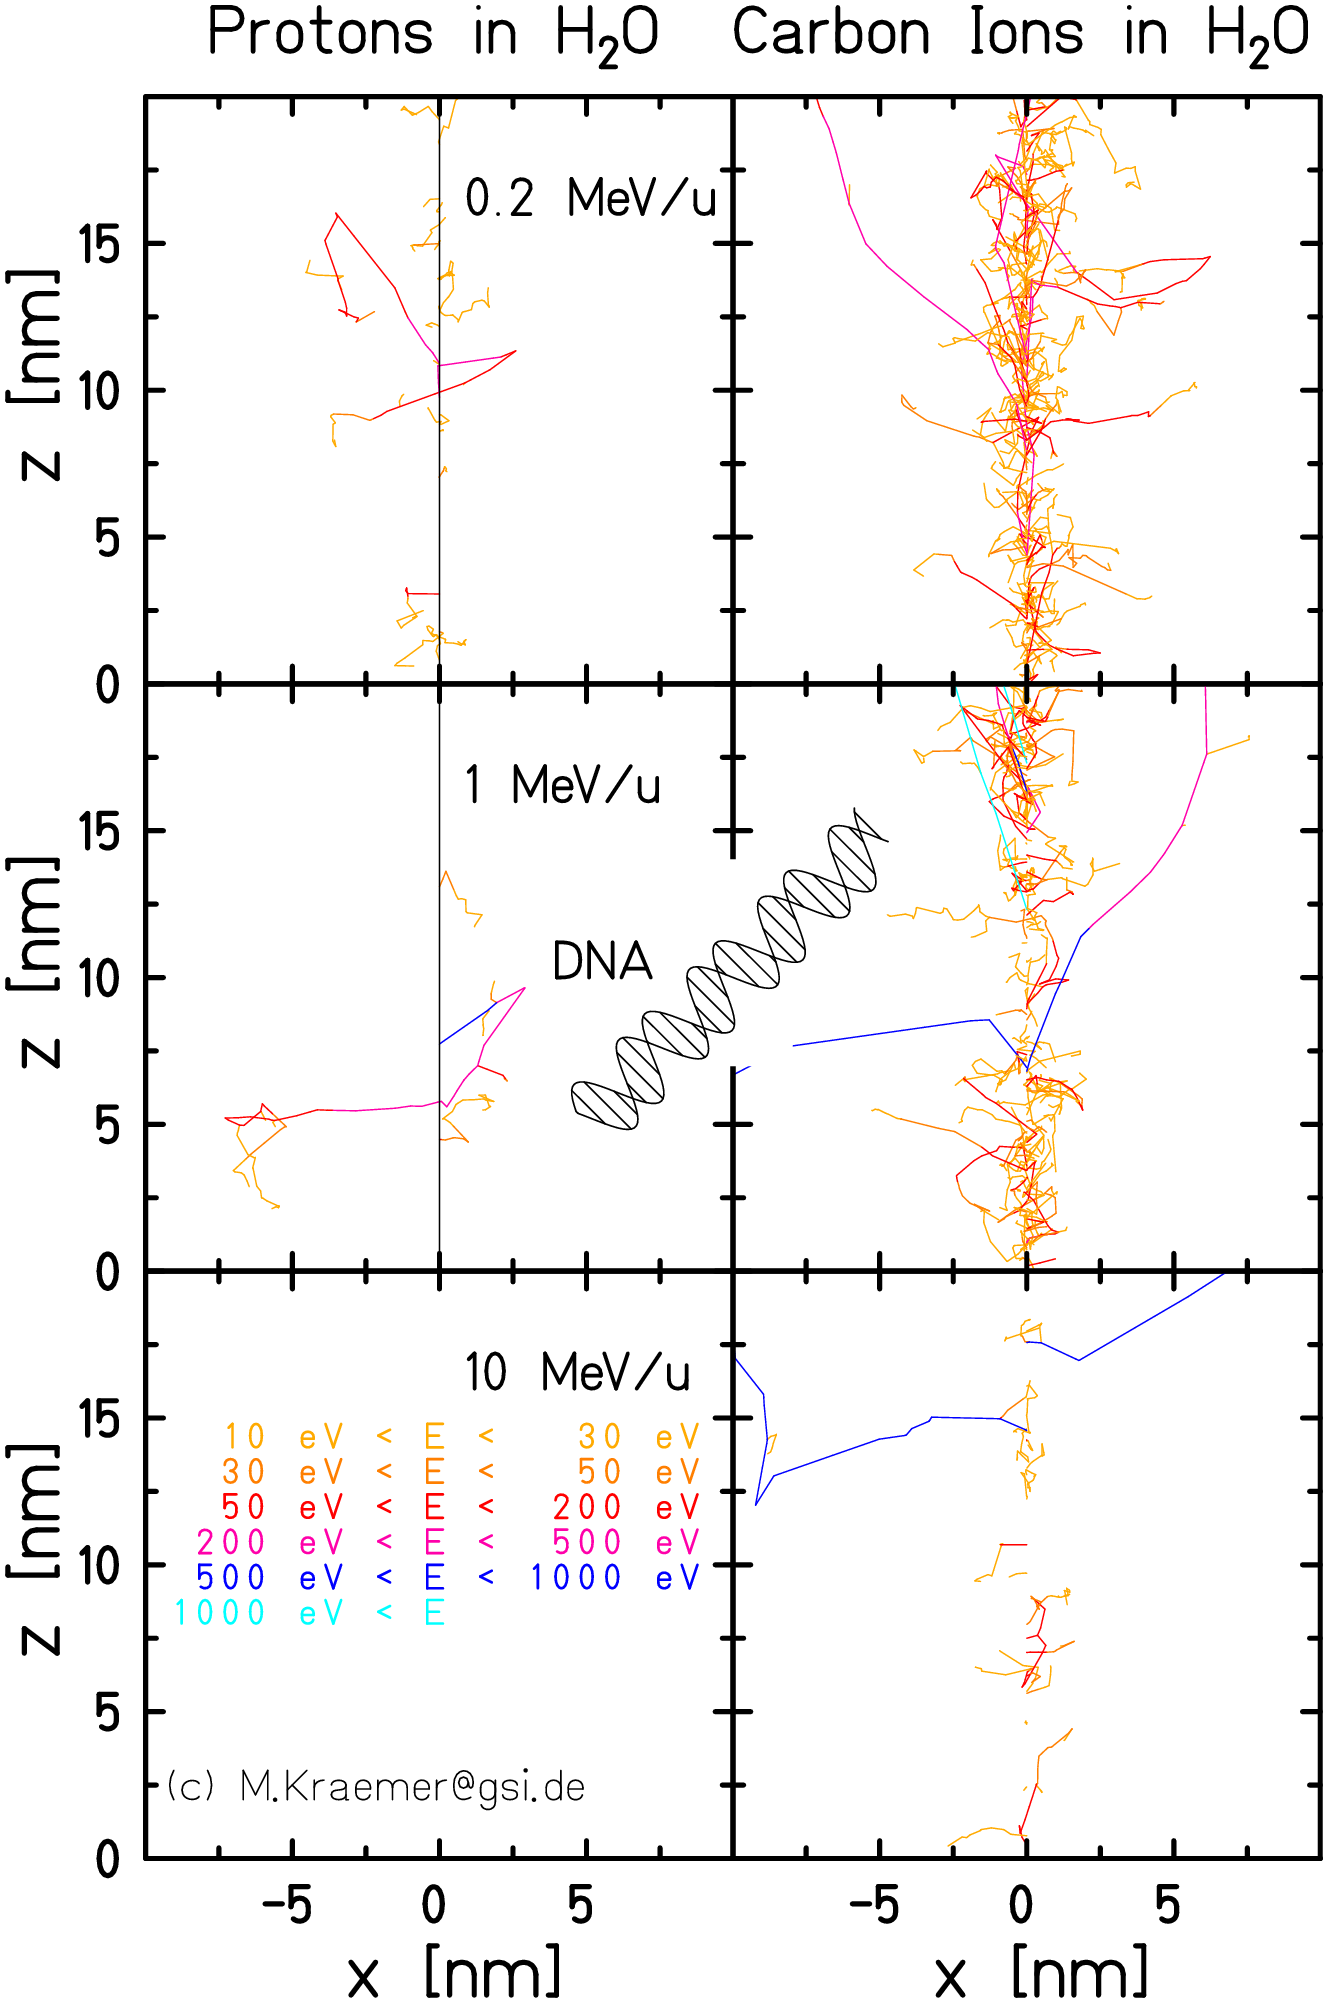
\includegraphics[width=0.8\textwidth]{./Images/trackstructure.png}
\caption{Track structure of ions in water at different energies. The distribution of $\delta$-electrons is highly dependent on ion species and their energy.
A molecule of DNA is displayed for size comparison. Figure courtesy of Michael Kr\"amer.}
\label{track}
\end{center}
\end{figure}


\begin{figure}[H]
\begin{center}
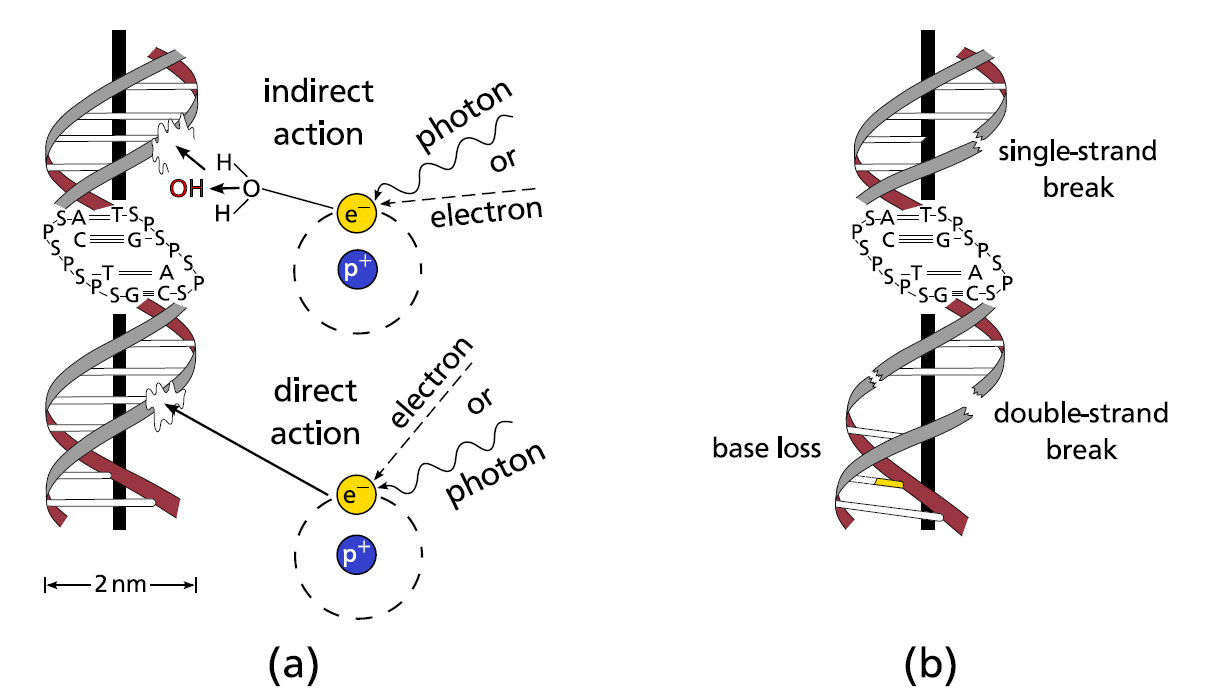
\includegraphics[width=0.9\textwidth]{./Images/SSB_DSB.png}
\caption{Types of DNA damage caused by radiation (a) Indirect damage occurs, when radiation forms free radicals hydroxyl radicals (OH), which can damage DNA. (b) Direct effects of radiation can cause single or double-strand breaks. 
Figure taken from \cite{Richter2012}}
\label{ida}
\end{center}
\end{figure}


Damage to DNA can result in either single strand breaks (SSB) or double strand breaks (DSB) as shown in Fig.~\ref{ida}b). When one of the double strands in the DNA helix is destroyed (SSB), it can usually be easily repaired by cell 
repair-mechanisms, since the complementary base is intact. If the bases on both stands are destroyed (DSB) the DNA damage is much more complex and can lead to the breakage of the chromatin. The cell repair-mechanisms can handle DSB as well, 
albeit not as efficient as SSB. However if there are clustered DSBs, the damage is usually too severe for repair-mechanisms to undo it. The changes in damaged DNA can lead to carcinogenesis or cell death. The aim of radiotherapy is to 
cause an apoptosis - a controlled self-inactivation of the cell due to the DNA damage. Beside apoptosis, cell can also undergo necrosis, an uncontrolled cell death. Cell necrosis often causes response from the immune system, leading to inflammation, which
radiotherapy strives to avoid. DNA can also be damaged to such extent, that cell cannot proliferate indefinitely - a effect known as clonogenic cell death.


\subsubsection{Relative Biological Effectiveness}
\label{RBE}

Fig.~\ref{track} shows the size of DNA molecule in comparison with proton and carbon ion distribution of $\delta$-electrons around their track. 
A clustered DSB occurs preferably around Bragg peak due to large ionization densities. Less cells will survive a clustered DSB, compared to DSB or SSB. Ions have large ionization density and is one of the main advantages over photons in the radiotherapeutic sense. Since most of the clinical experience about
cell response to radiation comes from photons, the biological effect of ions is usually described relative to a reference photon response. Relative biological effectiveness (RBE) is therefore defined as the ratio of the reference 
photon dose to the dose level of a specific ion radiation at the same biological effect (isoeffect):

\begin{equation}
 RBE = \left.\frac{D^{ref}_{photon}}{D_{ion}} \right|_{isoeffect}
\end{equation}

It is important to note at this point that RBE values are valid only for the same effect - the same biological endpoint and the same reference radiation. The most interesting biological endpoints in radiotherapy are cell survival and
side effects. RBE values are usually obtained from cell survival curves (see Fig.~\ref{dosedep}). Cell survival curves, S, are commonly modeled by an exponential linear-quadratic (LQ) model \cite{Fowler1989}:

\begin{equation}
 S(D) = e^{-\alpha D - \beta D^2}
 \label{lq}
\end{equation}

$\alpha$ is a coefficient related to a single event cell killing and $\beta$ coefficient related to a double event cell killing. The ratio of $\alpha / \beta$ is a characteristic of the cell type, namely the tissue 
capacity to repair radiation damage. A small $\alpha / \beta$ ratio means cell is radioresistive (high repair capacity) and vice versa.
As seen in Fig.~\ref{dosedep} and Eq. \ref{lq}, RBE values are dependent on the dose level. Hence in ion radiotherapy, beside the physical absorbed dose, a photo-equivalent or biological dose incorporating the RBE also plays an important role. 
The unit for biological dose is Gy (RBE) \cite{ICRU2007}. 

Besides a dose level, RBE also depends on the LET, the particle species and the tissue type \cite{Kraft2000}. Therefore RBE modeling is a complex topic.
At GSI, RBE is calculated using the \textit{local effect model} (LEM) developed by Scholz et al. \cite{Scholz1994}. There are two main assumptions in the LEM model. First is that localized biological 
effects are independent on the radiation type. Second assumption is that the photon response is the same for all dose levels (high and low).
The difference between different radiation types comes from the dose deposition in a small volume in the cell nucleus.
At the same total dose, many photons create a homogeneous dose distribution over a cell nucleus, while few ions cause a highly localized dose distribution around their track.

\newpage

\begin{figure}[H]
\begin{center}
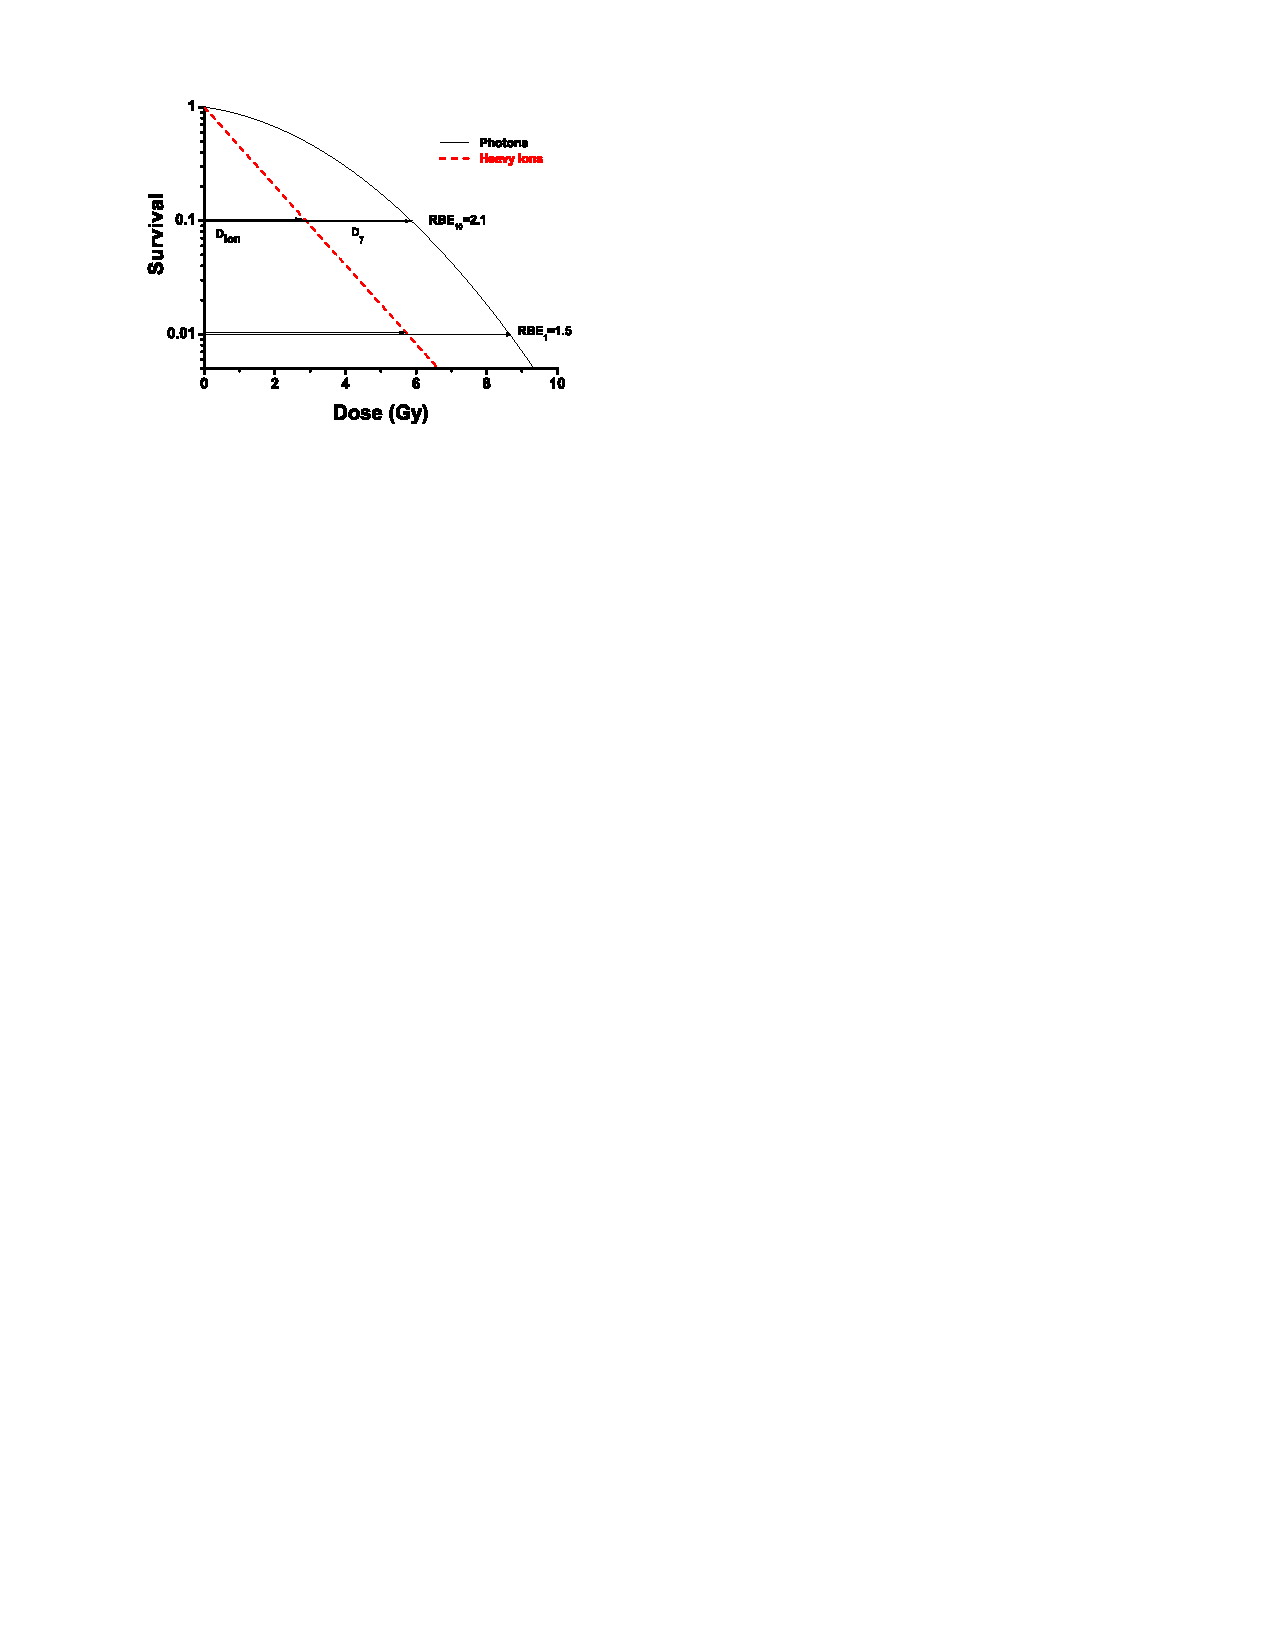
\includegraphics[width=0.6\textwidth]{./Images/dose_dependence.pdf}
\caption{Typical cell survival curve for photons (black solid line) and heavy ions (red dashed line). Photon line shows typical shouldered form, described by linear-quadratic model.
Heavy ions show a much steeper decrease with dose. The RBE value can be calculated by looking at the points at the same survival value - same biological effect. Figure taken from \cite{Schardt2010}}
\label{dosedep}
\end{center}
\end{figure}

 
LEM can thus predict dose response, by comparing
photon response at the high local dose level. LEM was used clinically as well in GSI pilot project from 1998 - 2007 \cite{Kraemer2000, Kraemer2000a} as in HIT since 2009. LEM has received several revisions \cite{Elsaesser2006, Elsaesser2007, Elsaesser2009} and experimental verifications
\cite{Mitaroff1998, Kraemer2000a, Kraemer2003}. 

RBE for carbon ions ranges from 1 in the entrance channel, to a value around 5 at 
the Bragg peak \cite{Kraft2000}. The highest RBE for carbon ions is right around Bragg peak, which gives carbon ions a great advantage, since there is an increased 
biological effectiveness at target tissue compared to the normal tissue in the entrance channel. In proton therapy a constant RBE value of 1.1 across the treatment field
is used \cite{Paganetti2002}.

\subsubsection{Fractionation}

Radiotherapy applies a basic principle of radiobiology that dose fractionation spares all cell types. For a given total dose
more cells will survive with dose delivered across multiple fractions, compared to a single dose, because cells will have time to repair
radiation induced sub-lethal damage between fractions.
With dose $d$ delivered over $n$ fractions, equation~\ref{lq} can be rewritten as \cite{Shrieve2011}

\begin{equation}
 S = (e^{-\alpha d - \beta d^2})^n
\end{equation}

The biologically effective dose (BED) is defined as:

\begin{equation}
 BED(Gy_{\alpha/\beta})=nd\left[1 + \frac{d}{\alpha/\beta} \right]
\end{equation}

with the total dose $D$ equal to $n \times d$, we can define fractionation factor $F$ as

\begin{equation}
 F = \left[1 + \frac{d}{\alpha / \beta} \right]
\end{equation}

so that BED = $D \times F$. $F$ increases with $d$, but decreases with $\alpha / \beta$. Lower $\alpha / \beta$ (late-responding tissue)
means higher $F$ and a higher $\alpha / \beta$ (early responding tissue) moves $F$ towards 1.


\subsubsection{Hypo-fractionation}

In recent years hypo-fractionation has showed promising results over wide range of tumors \cite{Yamada2008, Greco2011, Halasz2013}. 
Hypo-fractionation consists of 1-3 fractions of very high doses, up to 24 Gy in a single fraction (single-dose). The theory behind hypo-fractionation is still under research
and no consensus has yet been reached. On one hand, LQ model predicts higher BED for hypo-fractionation. On the other hand, Garcia-Barros et al. proposed additional mechanism at work \cite{Garcia2003}.
They presented a two target model, which suggest that tumor response to irradiation is defined not only by tumor cell type (as in LQ model) but also by micro-vascular
sensitivity. With excluding targeted enzymes from knock-out mice, they showed that tumors with reduced micro-vascular endothelial apoptosis grew 200-400 \% faster than a control group. The study, however, was challenged on several grounds and is controversal.
  

\subsection{Application technique}

The use of X-rays for treating patients has more than a century long history. There is a lot of research and practical knowledge regarding the clinical usage of X-rays. Particle therapy, on the other hand, is a more novel technique, with
more patients being treated every year. In the following sections an overview will be given of how the irradiation is actually delivered to the patient for both modalities with the emphasis on ion therapy.

\subsubsection{Photon therapy}

In photon therapy high energy x-rays (MV) are used for tumor irradiation. X-rays are produced in a linear accelerator (LINAC). Electrons are accelerated with energies from 2-25 MeV and collided with a high-density target (tungsten), where
x-rays are produced via bremsstrahlung. The beam is then directed to the patient and conformed to the tumor shape. The beam is shaped either by blocks at the head of the machine or by a multileaf collimator. A multileaf collimator is made of
individual leaves, that can be moved to represent the tumor's shape in the beam's eye view, see Fig.~\ref{MLC}.

Linear accelerators are usually placed on a gantry, which can be rotated around the patient. This allows beams to enter the patient from any angle. 
The arbitrary choice of beam angle is used in a 3-dimensional conformal radiotherapy, where a variable number of beams is used. 
Each beam is then shaped with a multileaf collimator. Even more precise technique is intensity-modulated radiotherapy (IMRT). IMRT allows treating complex tumor shapes, e.g. when the tumor is in proximity of a critical structure.
Volumetric modulatec arc therapy (VMAT) uses continuous irradiation together with continous gantry rotation and multileaf collimator shaping. VMAT is able to produce even more conformal dose shapes than IMRT.

\subsubsection{Ion therapy}

In order for ion therapy be successful, ions must be accelerated to appropriate energies (several hundred MeV/u), the beam must be transported to target area and guided
onto the target with the required accuracy.

\newpage

\begin{figure}[H]
\begin{center}
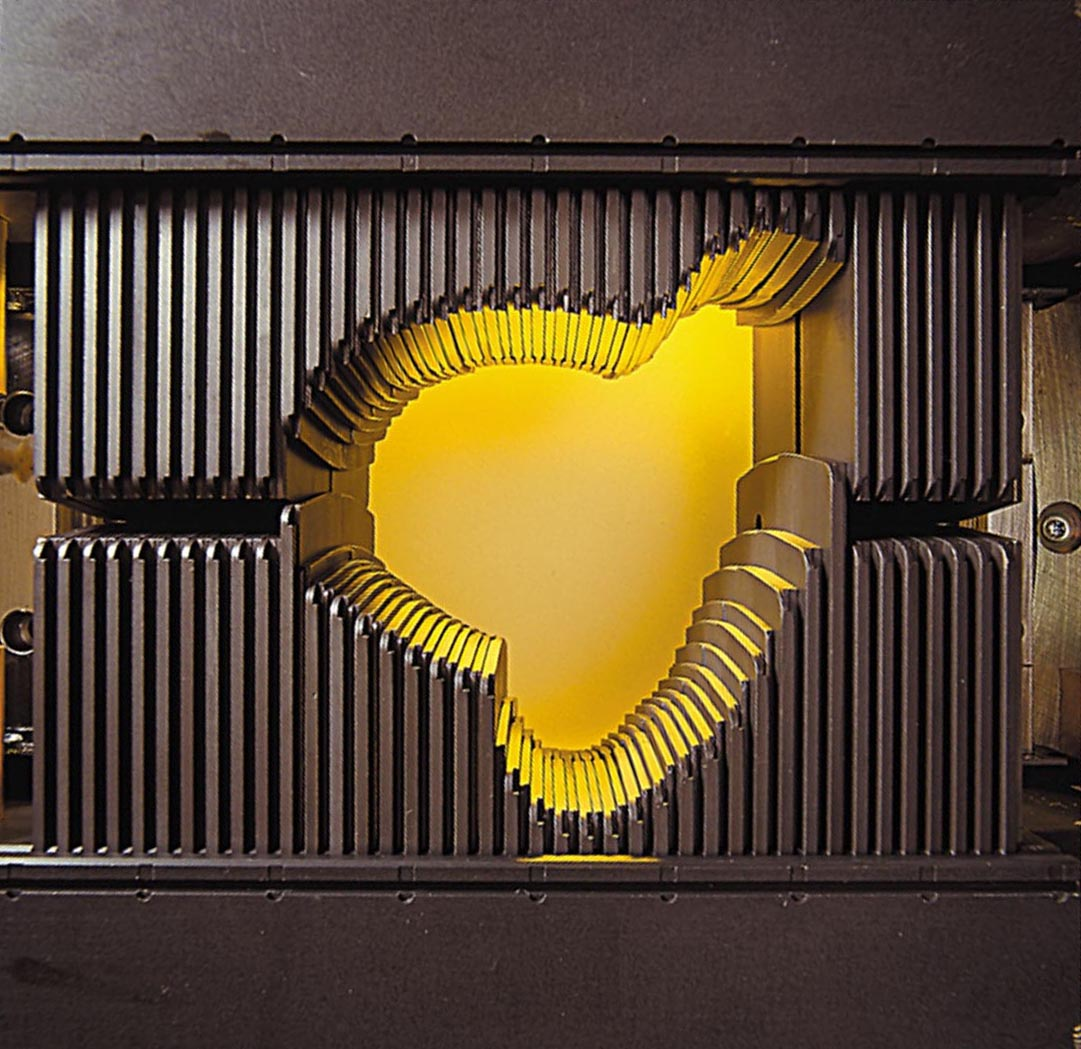
\includegraphics[width=0.7\textwidth]{./Images/MLC.png}
\caption{A schematic picture of a multileaf collimator. Individual leaves (marked with numbers) are positioned so that exit beam from linear accelerator conforms to the patient tumor in a beam's eye view. Picture taken from \cite{MLC}.}
\label{MLC}
\end{center}
\end{figure}

% \begin{figure}[H]
% \begin{center}
% 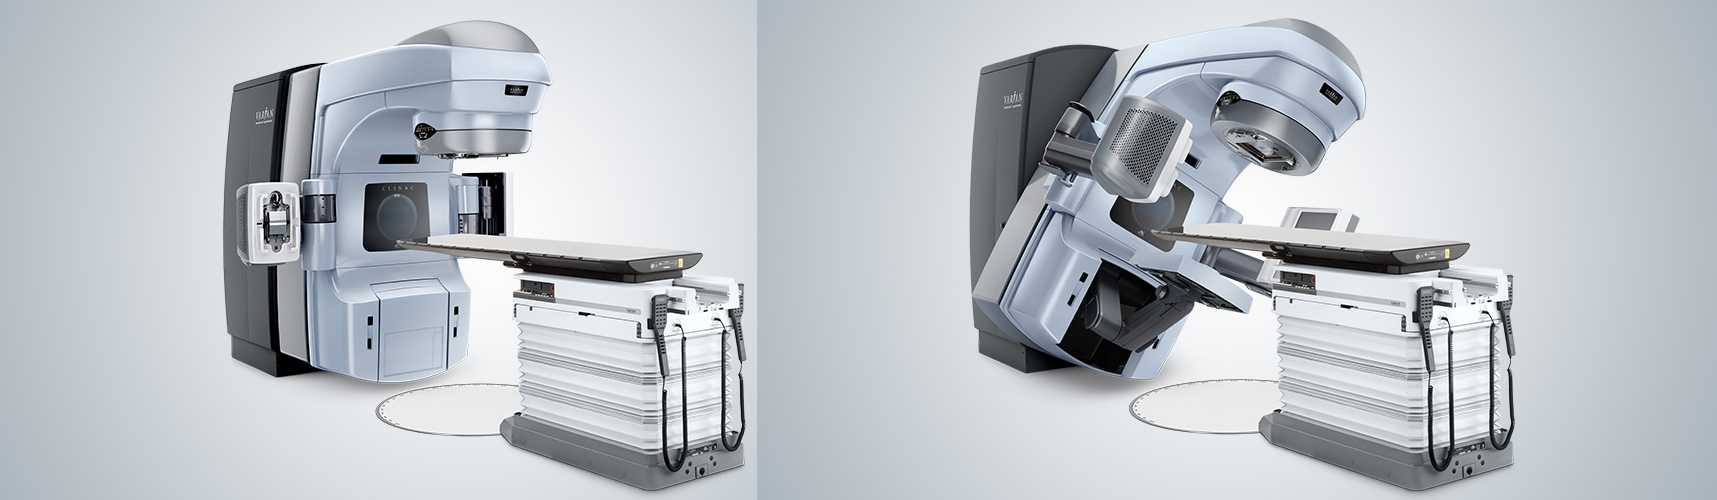
\includegraphics[width=0.9\textwidth]{./Images/gantry.png}
% \caption{A picture of a modern photon delivery system with gantry at two angles. Gantry can rotate 360 degrees around the patient. Picture taken from \cite{MLC}.}
% \label{gantry}
% \end{center}
% \end{figure}




Ion are accelerated either with cyclotrons or synchrotrons accelerators. \textbf{Cyclotrons} can be built in a compact design and offer a continuous beam with
stable intensities. Cyclotrons and only be used for protons and particle energies can not be regulated and therefore passive energy degraders are needed. Active energy variation is possible with \textbf{synchrotrons}, where a linear
accelerator is used to inject ions into the synchrotron and then the beam is regulated with ion optics. Synchrotrons are used in all heavy ion therapy centers, while cyclotrons are most
commonly used for proton therapy.

Each tumor has a unique shape, size and position in patient. Therefore a single Bragg peak would not provide adequate dose and a beam has to be properly shaped. Two beam shaping systems
are in use - passive and active beam shaping. In the next two sections both will be explained.


\subsubsection{Passive beam shaping}
\label{Sec::Passive}

The general idea of passive beam shaping is to transform a beam of a fixed single energy into the shape of the tumor. This is done in several steps as schematically shown in Fig. \ref{passive}. Firstly, the beam is broadened using a scattering device (passive double scattering systems or magnetic wobbler)
in order to obtain a broad, flat profile. In the next step, the beam is spread out over the required energy range with a range modulator. Usually a range modulator consist of rotating wheels of various thickness or a ridge filter \cite{Chu1993}. A beam of fixed energy is thus expanded into so-called \textit{spread-out Bragg peak (SOBP)}, which is moved to the required depth using a range shifter. The final two devices in beam's path are built for each patient individually. Collimator shapes beam in a lateral direction, while compensator adjusts SOBP to the distal edge of the tumor. However, compensator cannot adjust dose in the proxima ledge of the tumor, resulting in an access dose to the healthy tissue (hatched area in Fig. \ref{passive}).
 
Passive beam shaping offers more robust and faster treatment delivery in contrast to active beam shaping. However, it lacks tumor conformity, the dose cannot be modulated and each patient needs individually tailored devices for each beam used in the treatment.
 Furthermore, the beam travels through some material, exposing patient to additional dose due to fragmentation.

 \newpage
 
\begin{figure}[H]
\begin{center}
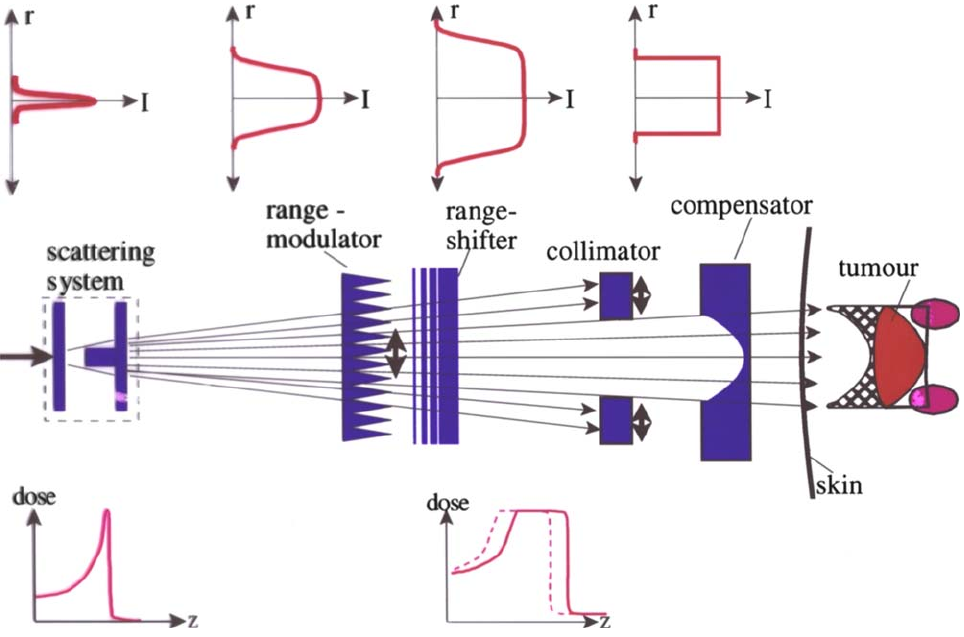
\includegraphics[width=0.7\textwidth]{./Images/deliverypassive.png}
\caption{Schematic presentation of a passive beam shaping. A scattering system is used to broaden the beam. Afterwards a range modulator spreads out Bragg Peak to the required energy range.
The spread out Bragg peak is then shifted to a specific energy with a range modulator. Finally, patient specific collimator and conformator serve for lateral and longitudinal conformity, respectively.
The proximal edge of the tumor cannot be shaped, as shown with hatched area. Figure taken from \cite{Schardt2010}.}
\label{passive}
\end{center}
\end{figure}

\subsubsection{Active beam shaping}
\label{Sec::Active}

In contrast to passive beam shaping, active beam shaping works by dividing tumor into small points, which are then irradiated using a thin pencil beam. Tumor is first segmented into iso-energy slices (IES) and each of IES
is covered with a 2 dimensional grid (raster points). A thin pencil beam is deflected from raster to raster point, irradiating each one with designated dose. The technique allows irradiation of arbitrary shape, without introducing any additional patient specific 
hardware. The lack of additional material in front of the patient also means less dose due to lesser neutron flux. Furthermore with the option to modulate dose in each point, dose in tumor is very conformal with less dose to healthy tissue.

There are differences in specifics of active beam shaping and the GSI system of three-dimensional scanning system will be given here \cite{Haberer1993,Kraft2000,Schardt2010} and a schematic presentation is shown in Fig.~\ref{scanning} and Fig.~\ref{active}.
A synchrotron provides a thin pencil beam of $^{12}$C ions with a variable energy in the range of 30 - 400 MeV/u. The energy defines the position of the Bragg peak in depth. Fig. \ref{active}b shows how the Bragg peaks are stacked in depth to cover longitudinal extension of the tumor.
The thin pencil is guided by two magnetic deflection units to irradiate each raster point. The specific dose in each raster point is calculated in the treatment planing.
During treatment the beam stays on each raster point until intensity monitoring system measures the designated dose. Then it is moved to the next raster point. When the whole IES is irradiated, the treatment waits for the next IES comes from accelerator.

Fig.~\ref{active}a displays how dose homogeneity in the target is achieved. To achieve flat dose distribution with Gaussian beam profile, beam's full width half maximum is three times the lateral raster spacing. Such configuration offers robustness for uncertainties of the beam spots.
The spacing between individual IES is usually 3 mm, providing enough overlap between individual Bragg peaks. However, the number of IES should be kept low, since the changing of the beam energy takes most of the time and hence prolongs the treatment. Instead of using high number of
 IES, Bragg peaks are broadened in longitudinal direction by a using ripple filter (RiFi) - a device similar to ridge filters used in passive beam shaping. 

\subsection{Motion in radiotherapy}
\label{sec:motion}

Patient motion can have a profound effect on the radiotherapy. It can cause large deviations from the planned dose, resulting in under- or over-dosage in target and excess dose in OAR. Motion types, its extent and origin is therefore a vast topic of research. 
A brief introduction will be given here, for an in-depth explanation reader is pointed to review by Langen and Jones \cite{Langen2001}.

\newpage

\vspace*{0.6cm}

\begin{figure}[H]
\begin{center}
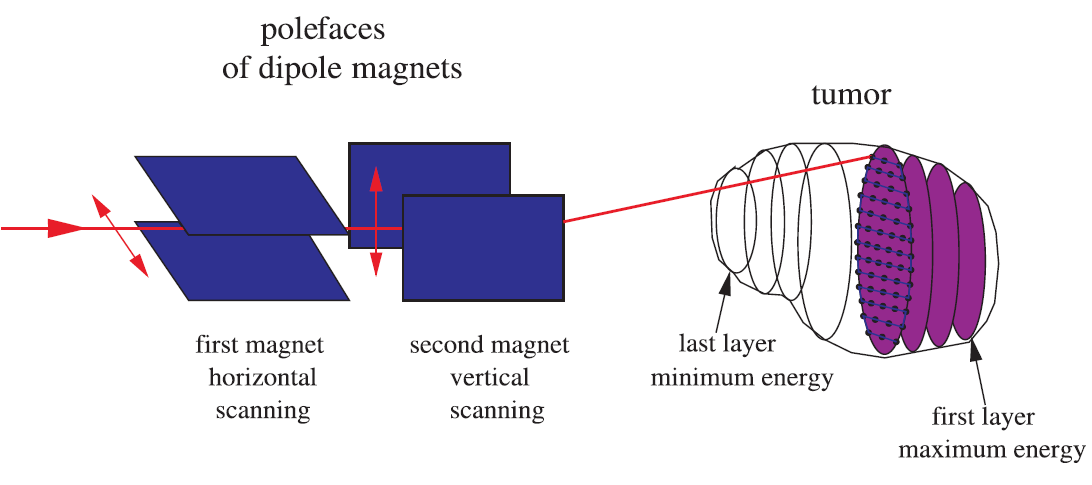
\includegraphics[width=0.9\textwidth]{./Images/therapy.png}
\caption{Schematics of GSI's active beam shaping. Tumor is divided into isoenergy slices, which are further overlayed with a 2 dimensional grid. 
Longitudinal direction (in beam's eye view) is varied with particle energy from accelerator, while lateral is via a magnetic scanning system. Figure taken from \cite{Kraemer2009}}
\label{scanning}
\end{center}
\end{figure}


\begin{figure}[H]
\begin{center}
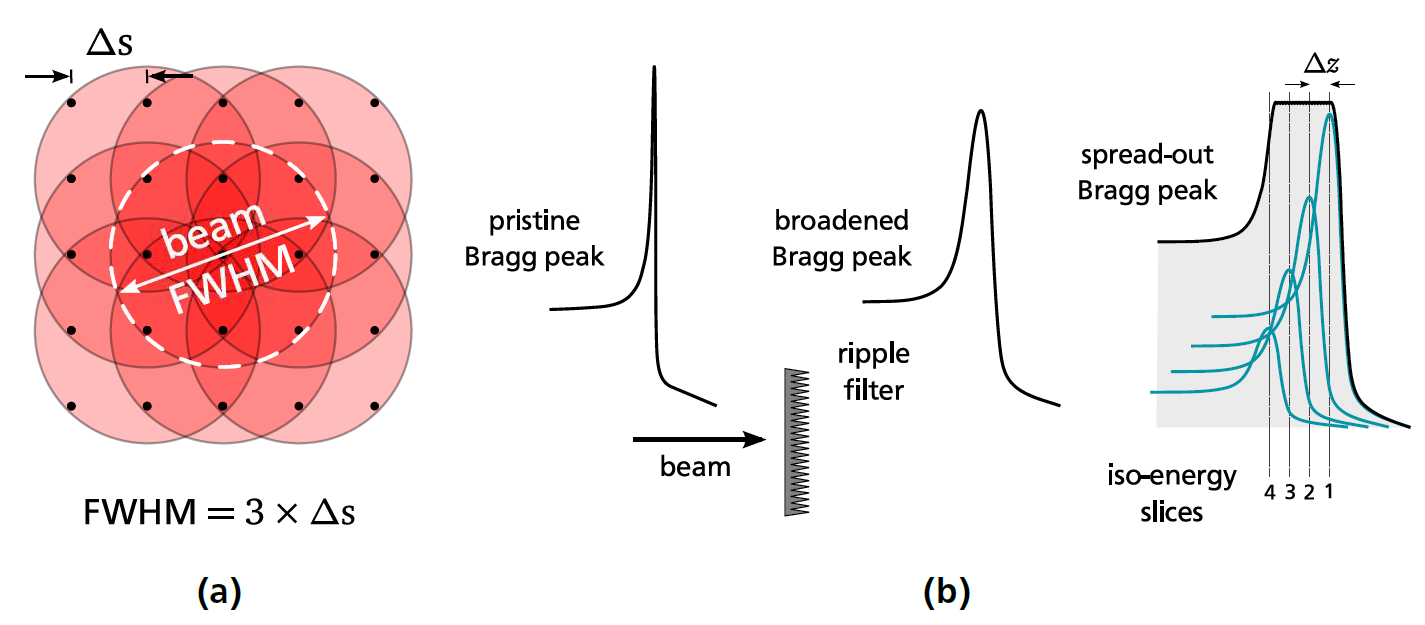
\includegraphics[width=0.9\textwidth]{./Images/active.png}
\caption{Schematic presentation of how target dose homogeneity is achieved in active beam shaping. a) To provide sufficient homogeneity in lateral direction (in beam's eye view) full width
half maximum of beam is three times the spacing between raster points. b) Bragg peaks are broadened in depth with a ripple filter and then stack to provide longitudinal dose homogeneity. 
Figure taken from \cite{Richter2012}}
\label{active}
\end{center}
\end{figure}


\newpage




\subsubsection{Motion types}

There are three main types of motion: patient positioning, inter- and intra-fractional motion. All three motion types are shown in Fig. \ref{motion}.
\newline
\textbf{Patient motion} is difference in patient position between image acquisition (e.g. CT) used for treatment planning and actual delivery. Patient motion introduces changes in tumor shape and tumor position. To overcome patient 
position uncertainties, patient immobilization and dedicated protocols are used.
\newline
\textbf{Interfractional motion} happens between two treatment sessions (fractions) and results in anatomical changes in a patient. It occurs on a time scale of hours and days. For lung cancer patients, tumor shrinks and lung density can change between fractions \cite{Mori2009}. 
Also changes in breathing pattern can impact treatment delivery. Additionally, the tumor baseline drifts significantly \cite{Sonke2008}. Repeated imaging and replanning reduces the impact of the interfractional motion, but requires additional time.
\newline
\textbf{Intrafractional motion} is mainly caused by respiration and heart beat, but also peristalsis. The time scale ranges from seconds to minutes. In this thesis we investigated treatment of lung cancer, so focus lies on respiratory motion. Respiratory motion varies from patient to patient and 
it is responsible for tumor motion from a mm range to a couple of cm \cite{Shirato2004a}. Tumor size and T-staging are also correlated to tumor motion \cite{Liu2007}. The respiratory-induced motion is largest in superior-inferior (SI) direction rather than 
in the anterior-posterior (AP) or left-right (LR) directions \cite{Seppenwoolde2002, Britton2007, Liu2007}.

\newpage

\begin{figure}[H]
\begin{center}
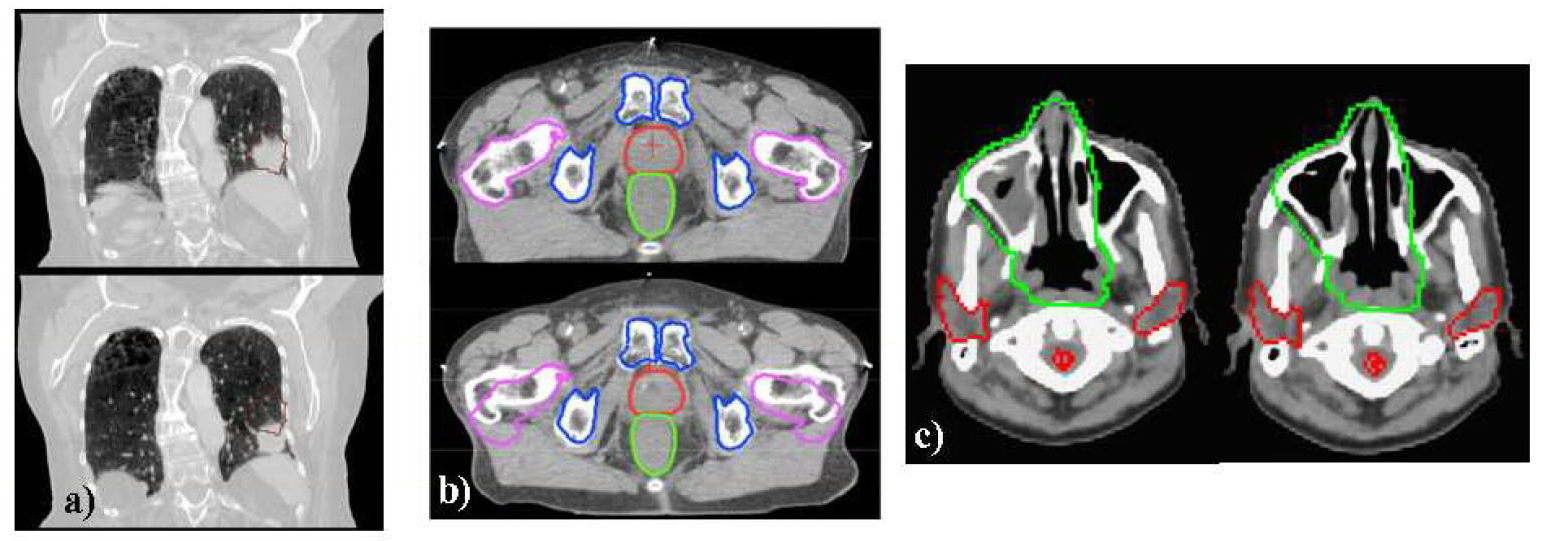
\includegraphics[width=0.9\textwidth]{./Images/motion_examples.png}
\caption{Examples of the three major motion categories. On the left side (a) a lung tumor is displayed, which moves due to the respiration 
of the patient (intrafractional motion). Interfractional position changes are exemplary shown in the middle (b), where two CT scans of a 
prostate patient are compared. Density variations between two CT scans are shown in (c). Figure taken from \cite{Engelsman2011}}
\label{motion}
\end{center}
\end{figure}

\subsubsection{Motion mitigation techniques}

While all three motion types have to be addressed in treatment planning, special focus will be given on intrafractional motion mitigation. Photon radiotherapy or particle radiotherapy with passive beam shaping 
use larger safety margins to encompass the whole tumor motion as explained in Section~\ref{treatmentPlanning}. However, larger safety margins are not enough to mitigate motion when active beam shaping is used. The beam delivery 
sequence and target motion interfere with one another, resulting in over- and underdosages in patients. This effect is called interplay and it has been thoroughly reviewed elsewhere \cite{Phillips1992,Bert2008}. The effect of interplay depends
on many factors, such as motion amplitude, beam direction, starting breathing phase etc. Three main techniques are currently established to counteract interplay: rescanning, gating and beam tracking. Several others techniques exist
to reduce the effect of tumor motion, such as abdominal compression, jet ventilation, apneic oxygenation etc., but will not be described here, since the scope of this thesis is on free-breathing patients.


\textbf{Rescanning} is a technique that uses statistical averaging of different interplay patterns \cite{Phillips1992}. Instead of applying the whole dose $D$ at once, the target is scanned $N$ times, each
time irradiated with $\mathrm{D}/\mathrm{N}$. The result is a Gaussian dose distribution around $D$ with no interplay (static case), as shown in Fig. \ref{rescanning}. With more rescans (larger $N$), better dose homogeneity is achieved, because the variance is proportional
to $\mathrm{1}/\mathrm{N}$. Technically the method is the easiest to implement of the three mentioned, since no real-time motion monitoring is necessary. The treated volume must be enlarged to at least encompass target in all motions states (in
contrast to gating), which introduces additional dosage to normal tissue. Rescanning is currently used at NIRS, Tokyo (Japan) and at \textit{some proton centers}.
\newline
\begin{figure}[H]
\begin{center}
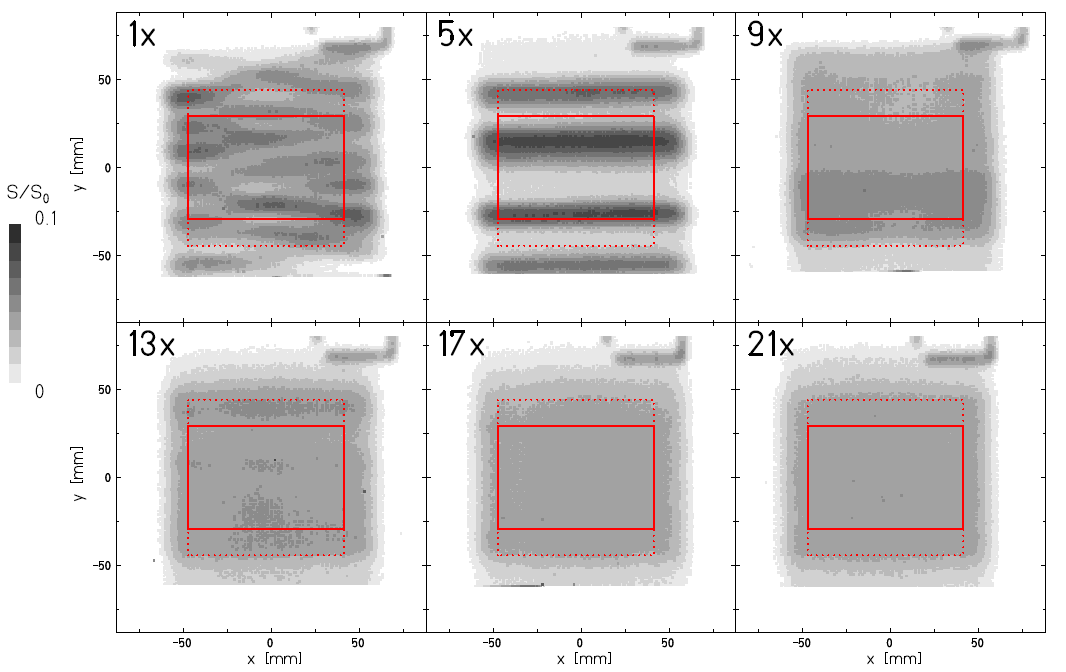
\includegraphics[width=0.7\textwidth]{./Images/rescanning.png}
\caption{Film irradiation with rescanning. With statistical averaging of multiple interplay patterns dose in the target (solid red square) becomes homogeneous. Figure taken from \cite{Bert2009}.}
\label{rescanning}
\end{center}
\end{figure}

\textbf{Gating} applies irradiation only in a selected part of the breathing cycle in a so-called gating window (GW) \cite{Minohara2000,Lu2006}. Usually, the end-exhale position is used as the center of the GW, as highlighted in Fig.~\ref{gating}.
A motion monitoring signal is used to control beam extraction. While there is limited additional normal tissue irradiation, the treatment time is prolonged due to frequent beam interruptions as shown in Fig. \ref{gating}.
Conventional radiotherapy and passive beam shaping also employ gating to reduce the effects of motion on treatment delivery.
\newline
\textbf{Beam tracking} is a method where the tumor is followed by the beam throughout different motion phases in real time. Similar to gating, beam tracking is not limited to active beam shaping. It was even proposed originally 
for photons \cite{Keall2001} and later implemented clinically in x-ray radiosurgery in the robotic Cyberknife Synchrony system (Accuray Inc., Sunnyvale, Ca., USA) \cite{Brown2007a,Kilby2010}. Regardless of radiation type, a
fast beam delivery system is required for beam tracking. In contrast to photon radiotherapy, beam tracking with particles need to pay special consideration to range changes. At GSI beam tracking system has been implemented.
The solution for fast longitudinal range changes was carried out by two polymethyl methacrylate (PMMA) wedges close to the target, that are operated via linear stepmotor \cite{Saito2009}, as shown in Fig.~\ref{tracking}. The stepmotor can
change the relative distance between the wedges and therefore introduces more or less material the beam travels through and consequently changes the effective beam energy (range). The beam position is corrected acording to the motion monitoring
signal and pre-calculated look-up tables for the required compenstation parameters. The beam tracking system at GSI is able to achieve high precision \cite{Bert2007, Bert2009, Saito2009}.
Clinical implementation, however, is not yet feasible due to several reasons, such as the precision and speed of the motion monitoring, the ion-beam tracking system complexity and inverse interplay.


The three motion mitigation techniques mentioned are not exclusive and can be used in parallel. Furukawa et al. made a study on a combination between rescanning and gating \cite{Furukawa2007} and Water et al. presented a combination
between rescanning and tracking \cite{Water2009}.

\begin{figure}[tbp]
  \centering
  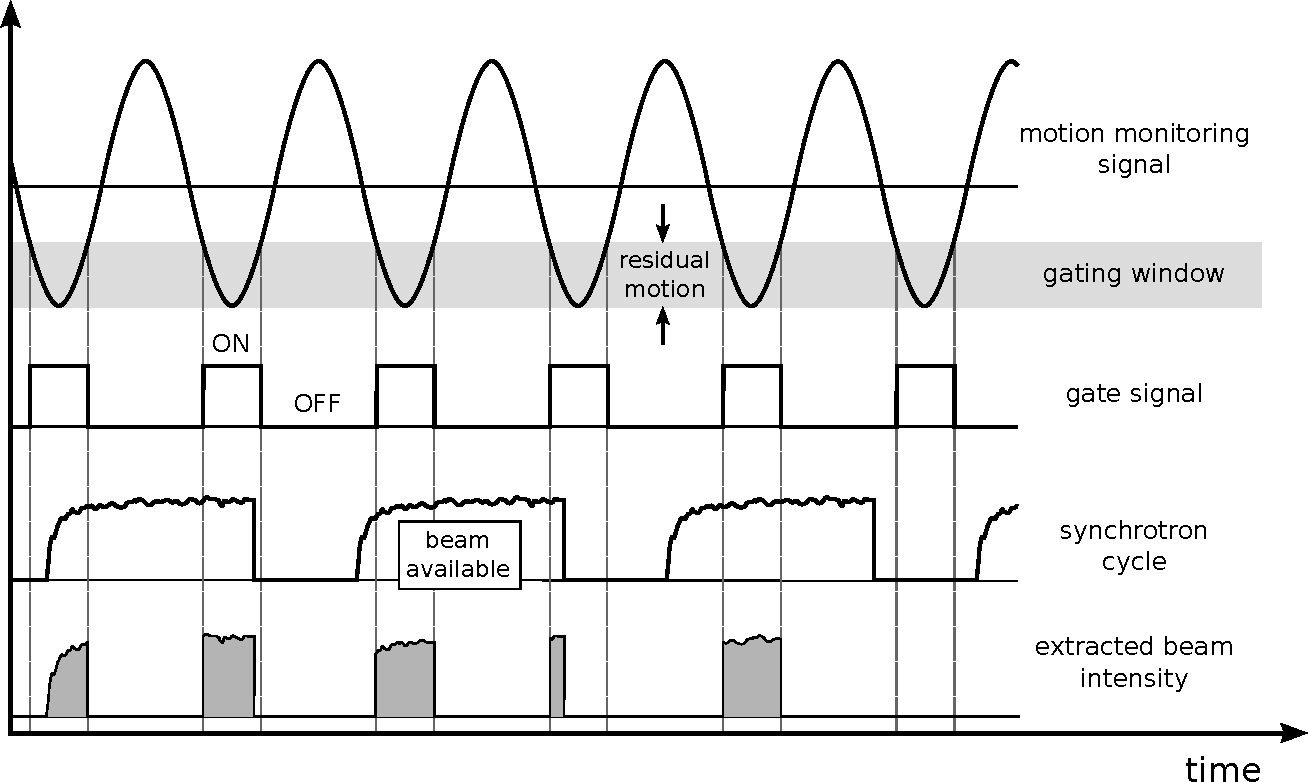
\includegraphics[width=0.9\textwidth]{./Images/gatingscheme.pdf}
  \caption{Gating delivery with a synchrotron accelerator. The irradiation is only possible, when the gate signal is active and the beam is available. The gate signal
  depends on gating window and motion monitoring signal. Figure taken from \cite{Richter2012}.}
  \label{gating}
\end{figure}

\newpage
\begin{figure}[H]
\begin{center}
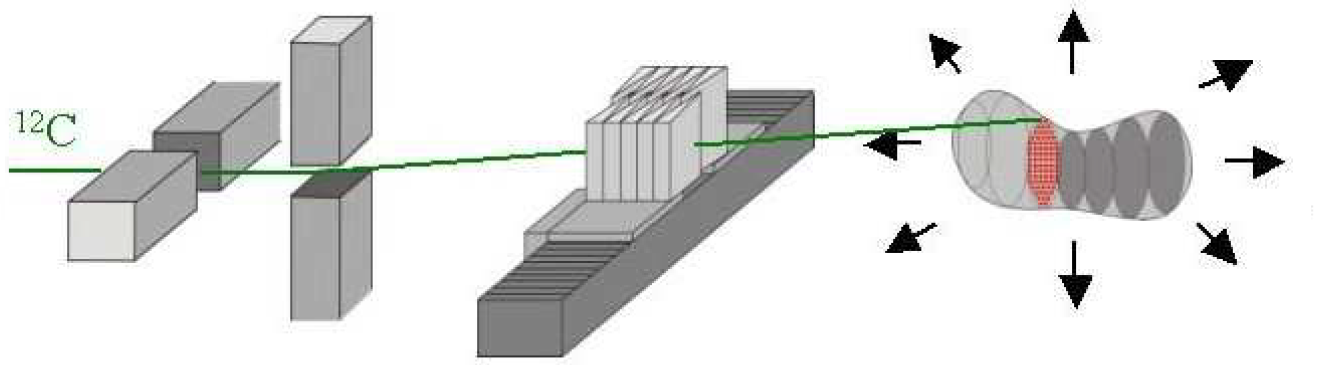
\includegraphics[width=0.9\textwidth]{./Images/tracking.png}
\caption{Schematic presentation of GSI's beam tracking system. Two PMMA wedges, mounted on linear stepmotor, can change the energy of the beam traveling through. The changes in lateral direction are achieved via dipole scanner magnets. For the longitudinal adaptation two 
PMMA wedges are mounted on step motors, enabling to change the depth the particle beam has to traverse. Figure taken from \cite{Groezinger2004}}
\label{tracking}
\end{center}
\end{figure}

\subsection{Treatment planning}
\label{treatmentPlanning}

The task of treatment planning is to determine machine parameters in order to deliver prescribed dose to the target, while not violating maximum allowed dose to critical organs, also known as organs at risk (OARs) \cite{Richter2012}.
Treatment planning thus revolves around dose optimization process and it is highly dependent on delivery type used for treatment. The optimization problem for tumors can be written as:

\begin{equation}
  \min_{x} \sum_{i} \left( f(x,A_i) - D_{pre} \right)^2 
\end{equation}

Here $i$ is a CT voxel, function $f$ is a dose deposition model, $x$ intensity of the radiation beams, $A$ patient geometry and beam parameters and $D_{pre}$ is the prescribed dose.

The basis of treatment planning is a computed tomography (CT), where target volume and OARs are delineated
done by physician. Additional imaging, such as magnetic resonance (MRI) or positron emission tomography (PET), is often used as a supplement to CT for enhanced contrast of it. In the following sections, the target definition will be explained and the basics of scanned ion beam treatment planning. Afterwards an explanation on dose calculation for moving targets will be given.

\subsubsection{Target definition}
The definition of the target volume is crucial, since it has to cover the whole tumor, prevent further tumor spreading, while at the same time it should not be too big to spare normal tissue. 
The International Commission on Radiation Units (ICRU) recommends the following definitions for volumes used in treatment planning, which will also be used in this work, see Fig.~\ref{targets} \cite{ICRU50, ICRU62}.
\begin{description}
\item[Gross Tumor volume:] \emph{The GTV is the gross
    palpable or visible/demonstrable extent and location of malignant
    growth.}
\item[Clinical Target Volume:] \emph{The CTV is a tissue
    volume that contains a demonstrable GTV and/or subclinical
    microscopic malignant disease, which has to be eliminated. This
    volume thus has to be treated adequately in order to achieve the
    aim of therapy, cure or palliation.}
\item[Planning Target Volume:] \emph{The PTV is a geometrical
    concept, and it is defined to select an appropriate beam size and
    beam arrangements, taking into consideration the net effect of all
    the possible geometrical variations, in order to ensure that the
    prescribed dose is actually absorbed in the CTV.}
\item[Internal Target Volume:] \emph{This is the margin that must be
    added to the CTV to compensate for expected physio-logical
    movements and variations in size, shape, and position of the
    CTV during therapy.}
\item[Organs at risk:] \emph{Organs at risk (OAR) are normal
    tissues whose radiation sensitivity may significantly influence
    treatment planning and/or prescribed dose.}
\end{description}

\begin{figure}[H]
\begin{center}
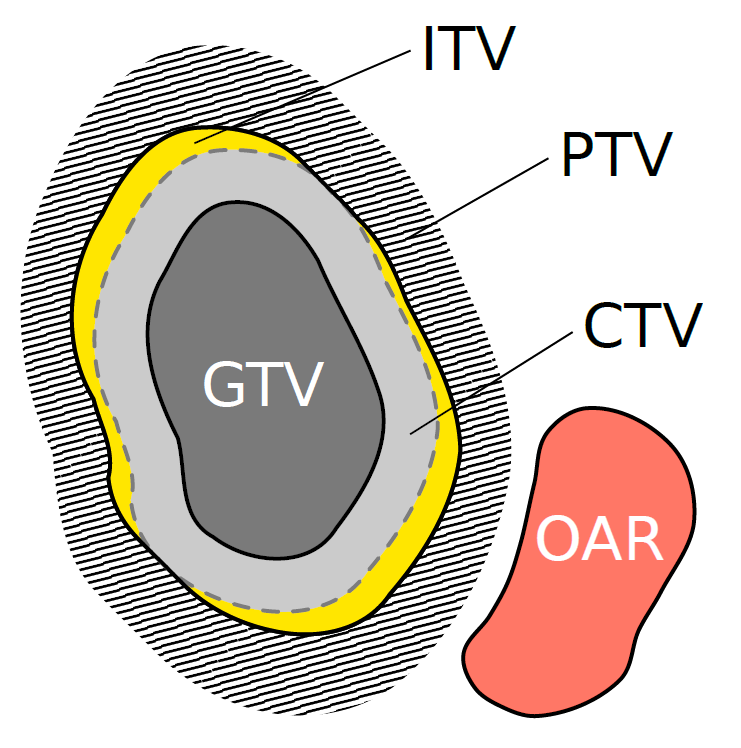
\includegraphics[scale=0.3]{./Images/volumes.png}
\caption{ICRU treatment planning volumes definitions. Figure taken from \cite{Richter2012}}
\label{targets}
\end{center}
\end{figure}

Further recommendations of the ICRU state that 100\% of the PTV volume should receive between 95\% and 100\% of the planned dose \cite{ICRU50}.


\subsubsection{Treatment planning for scanned ion beams}

A treatment planning system (TPS) for active shaping ion beams has to model the active beam delivery system and the beam interactions with the tissue. Furthermore, for ions heavier than protons
the biological effectiveness and fragmentation must also be considered, which add additional complexity to the TPS. A TPS for beam scanning was developed at GSI, called TRiP98. The basic concepts of TRiP98 will be
presented here, further reading can be found elsewhere \cite{Kraemer2000,Kraemer2000a, Richter2013}.

TRiP98 divides PTV into energy slices, which are further divided into raster points in a defined order that the beam will follow. In the optimization step, a gradient-decent algorithm iteratively optimizes particle number
for each raster point, so that the optimal target dose is achieved. Dose can either be physical or biological, using LEM biological effectiveness (see Section~\ref{RBE}).
Physical characteristic of the beam include lateral scattering as proposed by Moli\`ere \cite{Moliere1948} and nuclear fragmentation that yield secondary particles. The patient specific
geometry and tissue inhomogeneities are accounted for using a transformation from CT HU to water-equivalent path length (WEPL) \cite{Geiss1999,Jaekel2001,Rietzel2007}.


\subsubsection{GSI's 4D treatment planning system}

As mentioned in section \ref{sec:motion} tumor motion can cause severe dosimetric errors. To asses dose deficiencies and to overcome them, TRiP98 was expanded to be able to calculate time-resolved (4D) treatment plans. The new software was named TRiP4D and a detailed description is given by Richter et al \cite{Richter2013}.

A static CT is not sufficient for 4D treatment planning. Time-resolved CT scans (4D-CT) therefore have to be used. 4D-CT consist of several quasi-stationary sections, called motion phases. Data is
recorded in each slice throughout the whole motion and is then sorted to appropriate motion phases, according to motion signal \cite{Rietzel2005}.

Besides a 4D-CT, a vital part of 4D treatment planning is \textbf{image registration}. It provides quantification of motion with deformation maps between different 4D-CT motion states. Image registration principles are described in Section~\ref{sec:registration}. The image registration is not included in TRiP4D, so an external software must provide the necessary
deformation maps.

The calculation of 4D dose starts with the division of the treatment plan into sub-plans, according to the motion phase it will irradiate. The number of sub-plans is the same as number of motion phases (or number of motion phases
in gating window, if gating is used). Afterwards the number of particles is calculated in each voxel of all of the motion phases used. Finally, the particle number in each voxel is transformed with the deformation maps
obtained from registration, to the reference phase, where the accumulated dose from summed particle numbers is calculated (see Fig.~\ref{TRiP4Ddose}). If biological dose is calculated, then instead beside particle numbers, energy spectra is also accumulated, 
so that the RBE can be calculated according to LEM for the total dose to each CT voxel.

\begin{figure}[H]
\begin{center}
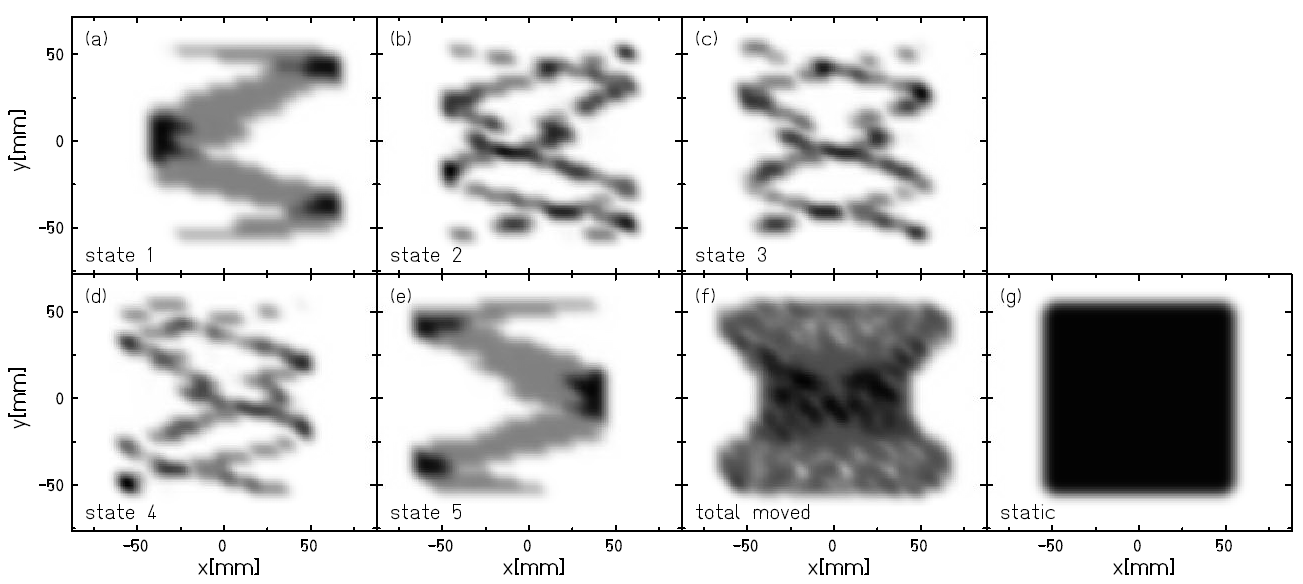
\includegraphics[scale=0.35]{./Images/4DtreatmentPlanning.png}
\caption{Experimental validation of TRiP4D dose calculation on film response. On images a)-e) the individual dose deposition for the five motion states is showed.
Image f) shows accumulated 4D dose and image g) a homogeneous dose on a stationary film. Figure taken from \cite{Richter2012}}
\label{TRiP4Ddose}
\end{center}
\end{figure}

\subsubsection{Image registration}
\label{sec:registration}


Temporal changes in patient anatomy are assessed with image registration. Registration can be made between different imaging modalities (CT, MRI, PET), between scans from different days or between
different phases in 4D-CT. It requires two images: a fixed and a moving one. The result of the registration is a deformation map originating from the moving and pointing to the fixed image. Registration can be written as:


\begin{equation}
\label{df}
x' = x + u_{ri}(x)
\end{equation} 

Here, $x$ and $x'$ are points in states $r$ and $i$, respectively and $u_{ri}$ is a vector field representation of the transformation map. $u_{ri}$ can be used to assess motion amplitude, propagate contours and calculate 4D dose.
It is important to note that certain steps in 4D treatment planning require also inverse registration, from state $i$ to $r$ \cite{Richter2012}. If deformation map is applied to the moving image, 
the new image is called warped image and it should be as close to the fixed image as possible. Fixed, moving and warped image are shown in Fig.~\ref{RegistrationCompare}. 

\begin{figure}[H]
\begin{center}
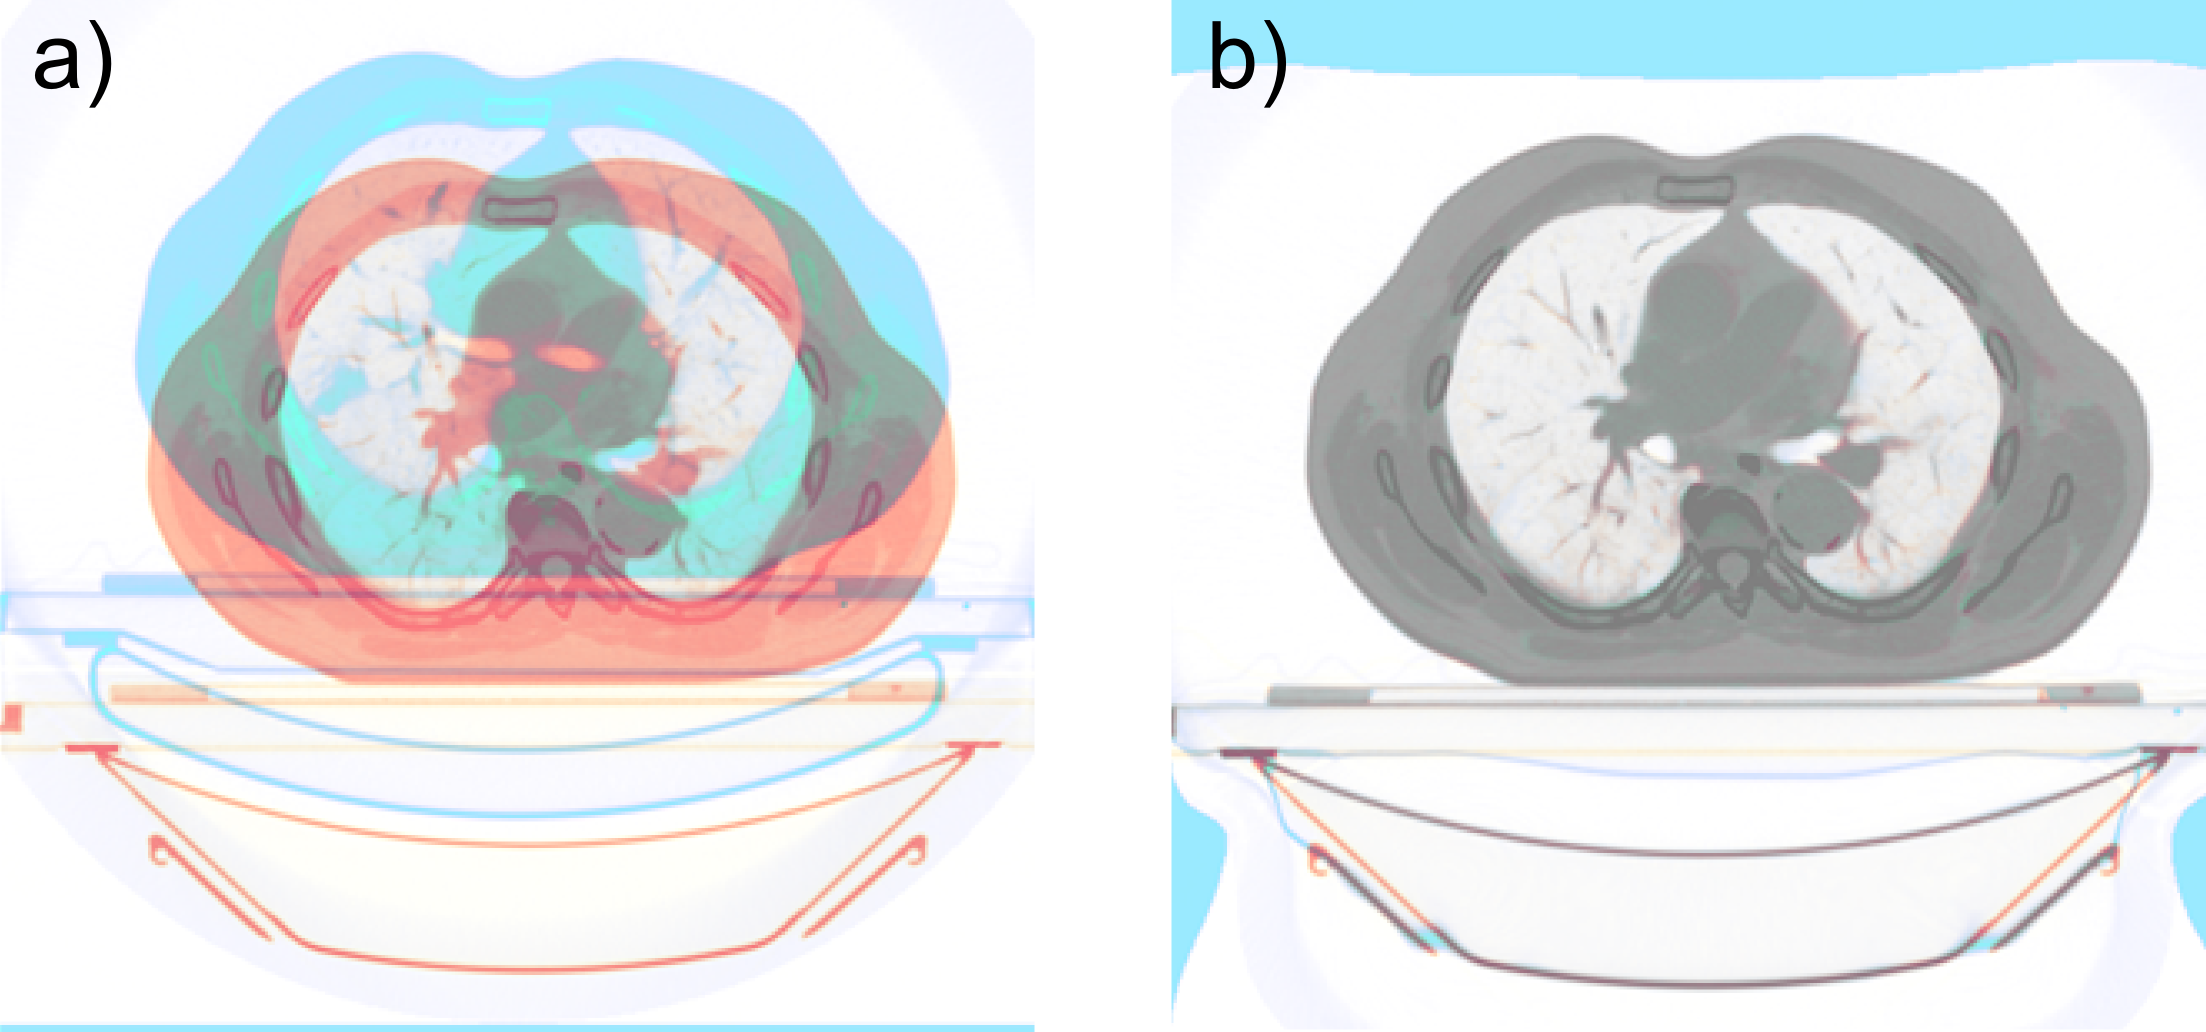
\includegraphics[width=0.9\textwidth]{./Images/RegistrationCompare.png}
\caption{Overlap of fixed and moving image CT scan (a) and fixed and warped image after registration (b). Inverse colors are used in both CTs so that the overlayed image should be gray
where the images overlap perfectly.}
\label{RegistrationCompare}
\end{center}
\end{figure}

There are different possible types of registration and can be placed in two groups. First group consist of linear registrations: translation, rotation and scaling. In medical imaging the most commonly used linear transformation 
is translation or rigid registration. The other group of registrations are elastic or deformable registrations. The actual algorithms for performing registration are complex and the reader can
find detailed review elsewhere \cite{Hill2001,Brock2006,Rietzel2006a}. A multi-institutional study has shown that the accuracy for the majority of the algorithms is in the order of image voxel
size, i.e. millimeters \cite{Brock2010}. The study further states that the registration quality depends on image contrast. The quality of image registration is actually hard to quantitatively
asses and usually the registration results are checked visually. To improve image registration quality assurance a dedicated software was developed and is described in detail in chapter \textbf{REF}.

\newpage




\section{Lung cancer}

There were 1.8 million new lung cancer cases diagnosed worldwide in 2012 \cite{Worldwide2012}. With a very poor prognosis (5-year survival rates in Germany are
16\% for men and 21\% for women \cite{Kaatsch2014}) lung cancer is one of the most frequent and most deadly cancer types. Usually lung cancer is distiguised
into small-cell lung cancer (SCLC) and non-small cell lung cancer (NSCLC). Around 14\% of lung cancer cases are SCLC \cite{Tsao2008}, which is normally treated with chemotherapy and radiotherapy, while for NSCLC the traditional course of treatment
are surgery and radiotherapy. An example of cancerous lung tissue is shown in Fig.~\ref{Fig:Cancer}.

\begin{figure}[H]
\begin{center}
\includegraphics[width=0.7\textwidth]{./Images/LungCancer.png}
\caption{Cross section of a human lung. The white area in the upper lobe is cancer, the black areas indicate the patient was a smoker. Figure taken from \cite{LungCancer}}
\label{Fig:Cancer}
\end{center}
\end{figure}


\subsection{Epidemiology}

The main cause for lung cancer is a long-term exposure to tobacco smoke \cite{Tsao2008}, with 85\% of cases contributed to smoking. There are over 70 known carcinogens in cigarette smoke, such as benzo[a]pyrene, 1,3-butadiene and a radioactive isotope of polonium, polonium-210 \cite{Hecht2012}. See Fig.~\ref{Fig:Smoking} for correlation between sales of tobacco products and rate of the lung cancer.

Studies have shown that passive smokers have an increased risk of lung cancer as well, with more then 20\% increase in risk for those who live with someone who smokes and 16-19\% increase for someone working with a smoker \cite{Taylor2007}.
There is some controversy weather smoking cannabis increases risk of lung cancer - two reviews from 2013 and 2014 have found contradicting results \cite{Tasckin2013, Underner2014}.

The other 15\% of lung cancer cases is attributed to a combination of genetic factors, exposure to radon gas, asbestos or other forms of air pollution \cite{Alberg2010}.

\begin{figure}[H]
	\begin{center}
		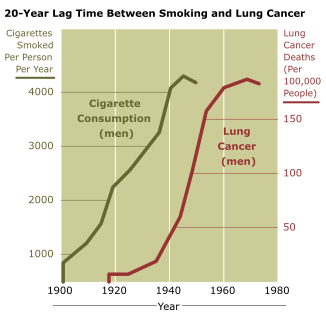
\includegraphics[width=0.7\textwidth]{./Images/Smoking.png}
		\caption{Correlation between sales of tobacco products and the rate of the lung cancer in the USA between 1900 - 1970. Data released from National Cancer Institute.}
		\label{Fig:Smoking}
	\end{center}
\end{figure}


\subsection{Non-small cell lung cancer}

The NSCLC is divided into three main groups: adenocarcinoma, squamous-cell carcinoma and large-cell (undifferentiated) carcinoma \cite{Kasper2015}.
Between 25-35\% of all lung cancer cases are adenocarcinoma, squamous-cell carcinoma contributes to around 30\% of lung cases and 10-15\% are large-cell carcinoma. The SCLC contributes the rest. 

Lung cancer staging is used to refers to the extent to which the lung cancer has to spread from it's original source. Additionally, staging is used to establish treatment and prognosis \cite{Chheang2013}. For NSCLC, the TNM classification is used, which depends on
size of the primary tumor (T), involvement of the lymph node (N) and distant metastasis (M) \cite{Kasper2015}. According to the TNM class a group is assigned, from stage 0, IA, IB, IIA, IIB, IIIA, IIIB to IV. 
A schematic presentation of some stages is shown on Fig.~\ref{Fig:Stages}. Prognosis is highly dependent on stage, as shown in Table~\ref{tab:prognosis}.

\begin{table}[H]
  \centering
%   \footnotesize
  \caption{Five-year survival rates for different stage of NSCLC. Data taken from \cite{Rami2009}}
  \begin{tabular}{|c|c|}
   \hline
   \hline
Clinical stage & Five-year survival (\%) \\
IA & 50 \\
IB & 47 \\
IIA & 36 \\
IIB & 26 \\
IIIA & 19 \\
IIIB & 7 \\
IV & 2 \\
\hline
\hline
  \end{tabular}
  \label{tab:prognosis}
\end{table}

\begin{figure}[H]
\begin{center}
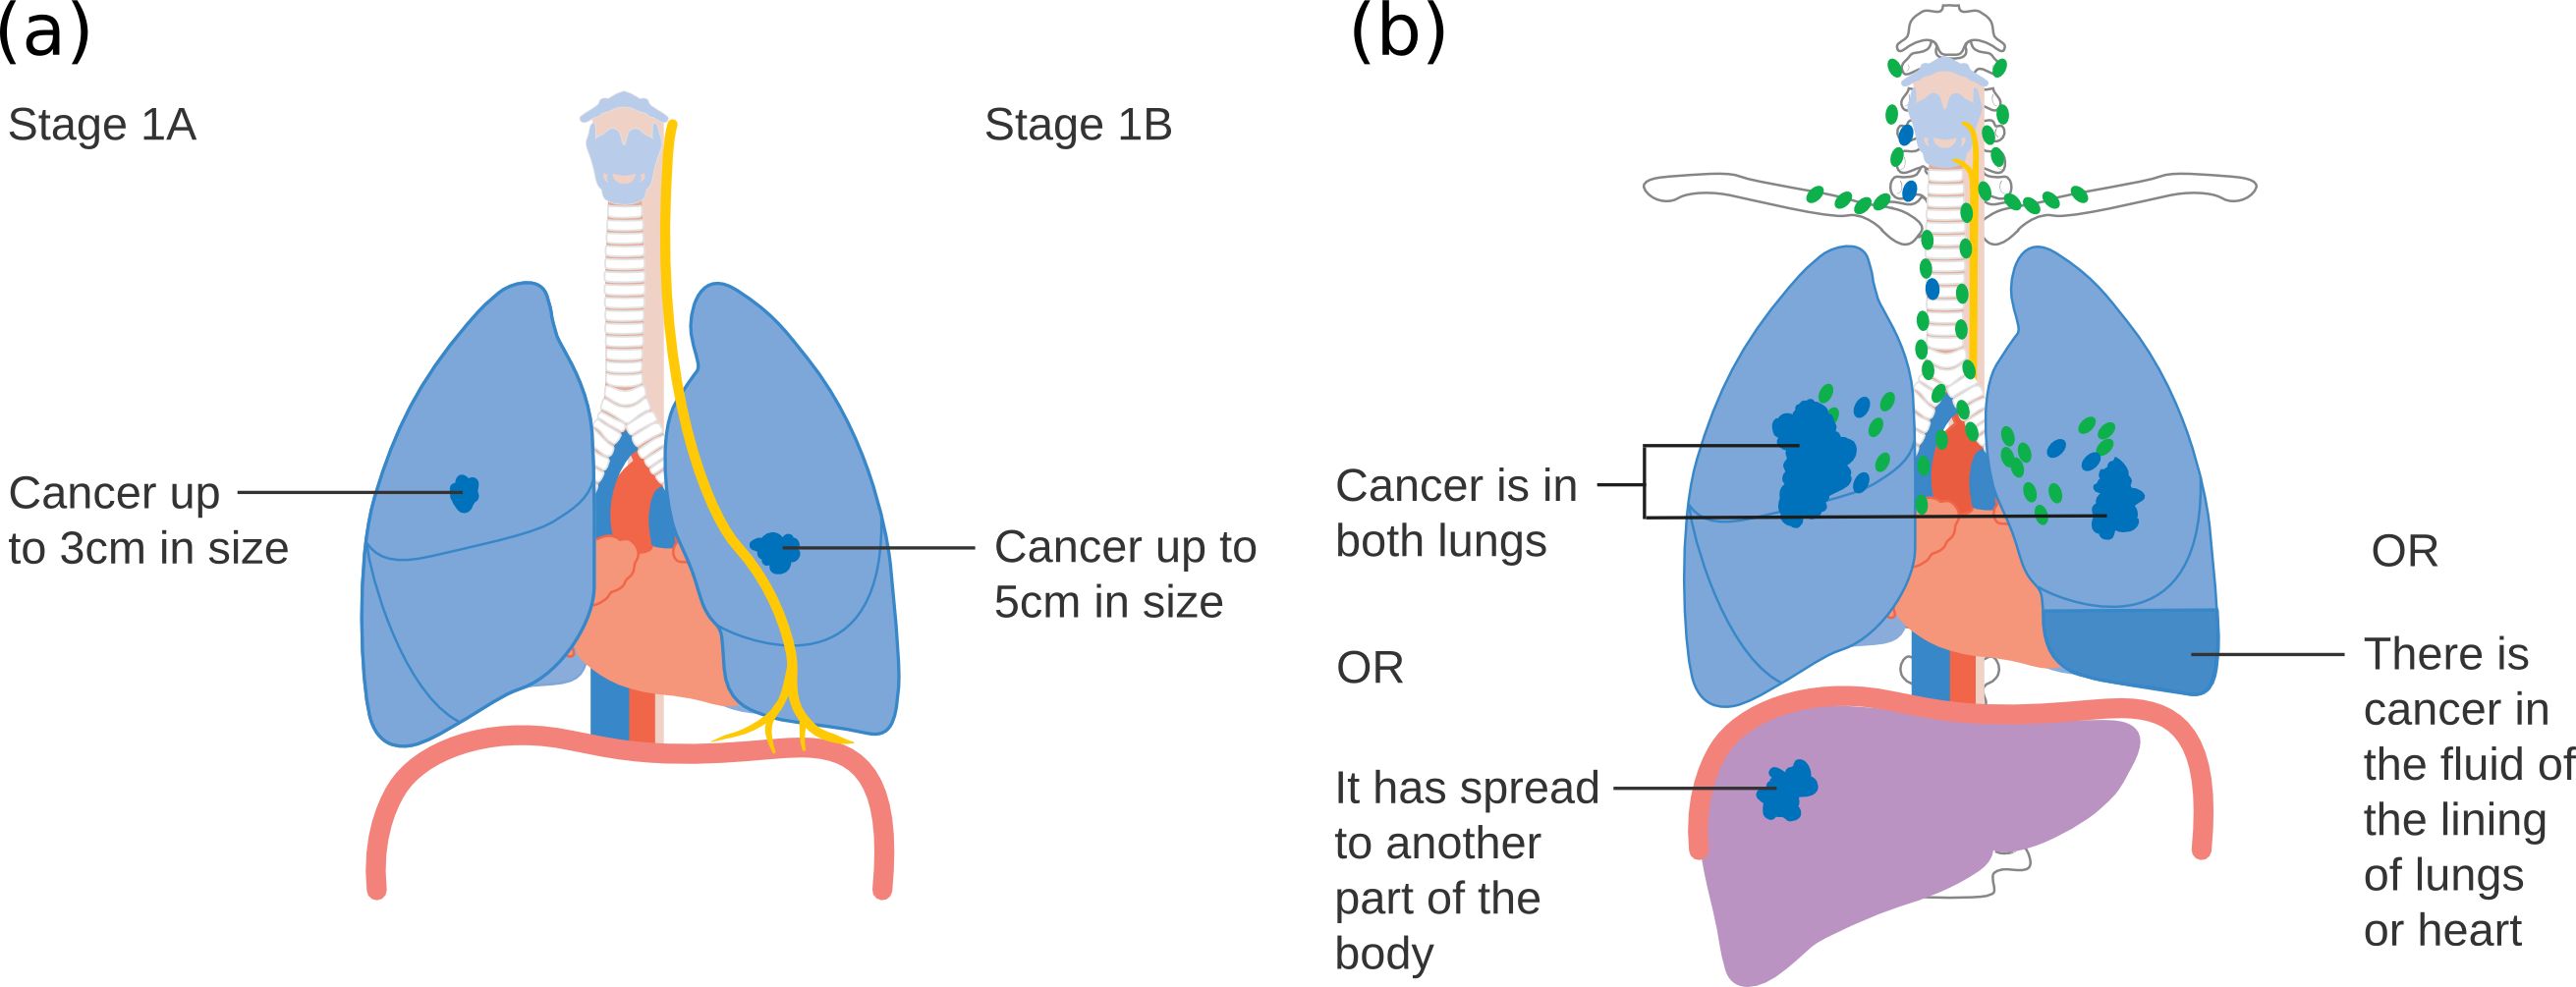
\includegraphics[width=0.9\textwidth]{./Images/Stages.png}
\caption{Schematic presentation of three NSCLC stages. (a) Stages IA and IB; (b) Stage IV. Figure taken from \cite{CancerStage}}
\label{Fig:Stages}
\end{center}
\end{figure}

\subsubsection{Treatment}

The treatment for NSCLC can consist of surgery, chemotherapy, radiation therapy, or a combination of modalities. The treatment course depends on tumor type and stage and on patient overall condition
The typical treatment is surgery for stage I and II disease \cite{Tsao2008}. Surgery resection consist of either lobectomy or pneumonectomy, together with sampling lymph node or even a complete lymph node
dissection. Surgery will only be performed if NSCLC patients have enough lung reserve after lobe or lung is removed. The 5-year survival rate for NSCLC patients undergoing surgery is about 55 to 70\% 
and 35-55\% for stage I and II disease, respectively.

For unresectable stage III lung cancer the treatment consist of either chemotherapy or radiation therapy or a combination of both. The median survival for patients with unresectable stage IIIA disease is 10-14 months \cite{Tsao2008}.
For all treated stage IIIB disease the median survival is 7-15 months \cite{Srisam2005}.

Rather than treating stage IV disease, palliation of symptoms is the goal. With chemotherapy, targeted drugs and radiation therapy the tumor burden can be lessened and the quality of life can be improved. The prognosis is poor, with
median survival only 9 months and less then 25\% survive the first year after the disease is diagnosed \cite{Tsao2008}. Recent phase II trial combined chemotherapy with stereotactic body radiation therapy and 
showed promising results with 20 months overall survival \cite{Iyengar2014}.


\bibliographystyle{apalike}
\bibliography{../ref.bib}{}
% \bibliographystyle{plain}

\end{document}
